\documentclass{article}
\usepackage[T1]{fontenc}
\usepackage[latin1]{inputenc}
\usepackage{textcomp}
\usepackage{amsthm}
\usepackage{amsmath}
\usepackage{amssymb}
\usepackage{graphicx}
\usepackage{subfig}
\usepackage[letterpaper]{geometry}
\geometry{verbose,tmargin=4cm,bmargin=3cm,lmargin=3cm,rmargin=3cm}
\usepackage{fancyhdr}
\pagestyle{fancy}
\usepackage{algorithm,algorithmic}
\usepackage{tikz}
\usepackage{verbatim}
\usetikzlibrary{arrows,shapes}
\usetikzlibrary{decorations.pathmorphing,trees}

\usepackage{pst-all}



%%%%%%%%%%%%%%%%%%%%%%%%%%%%%%%%%%%%%%%%%%%%%%%%%%%%%%%%%%%

\theoremstyle{plain}
\newtheorem{theorem}{Theorem}
\newtheorem{algo}{Algorithm}
\newtheorem{problem}{Problem}
\newtheorem{definition}{Definition}
\newtheorem{lemma}{Lemma}
\newtheorem{claim}{Claim}
\newtheorem{prop}{Proposition}
\newtheorem{corollary}{Corolary}
\newtheorem{conj}{Conjecture}

\theoremstyle{remark}
\newtheorem*{example}{Example}
\newtheorem*{remark}{Remark}

\floatname{algorithm}{Algorithme}


\newsavebox{\fmbox}
\newenvironment{encadre}[1]
{
\begin{lrbox}{\fmbox}
\begin{minipage}{\textwidth-3em}
\vspace{0.3\baselineskip}\setlength{\parskip}{0.5em}
}
{
\vspace{\baselineskip}
\end{minipage}\end{lrbox}
\begin{center}
\fbox{\hspace{1em}\usebox{\fmbox}\hspace{1em}}
\end{center}
\vspace{0.5\baselineskip}
}

\numberwithin{equation}{section}

%%%%%%
\newcount{\vari}
\newcount{\lin} %pour les put
\newcounter{nbr} %pour l'affichage
\newcounter{prog} %num prog
\setcounter{prog}{0}

\newenvironment{Algo}[1]{
\setlength{\unitlength}{1mm}
\begin{picture}(0,0)(0,2)
\lin=0
\setcounter{nbr}{0}
\Algotitle{#1}
}
{
\Algoend
\end{picture}
}
\newcommand{\Algotitle}[1]{
\addtocounter{prog}{1}
\put(2,-3.5){\textbf{Algorithm \theprog.} #1}
\linethickness{0.8pt}
\put(0,\lin){\line(1,0){130}}
\linethickness{0.3pt}
\advance \lin by -5
\put(0,\lin){\line(1,0){130}}
\advance \lin by -2
}

\newcommand{\algoline}[1]{
\advance \lin by -4
\addtocounter{nbr}{1}
\ifnum \thenbr<10 \vari=4 \else \vari=2 \fi
\put(\vari,\lin){\thenbr}\put(10,\lin){#1}
}

\newcommand{\Algoend}{
\linethickness{0.3pt}
\advance \lin by -4
\put(0,\lin){\line(1,0){130}}
}

\newcommand{\Algospace}[1]{
\lin=#1
\advance \lin by 3
\multiply \lin by 12
\begin{picture}(0,\lin)(0,0)
\end{picture}
}

\newcommand{\tab}{$~~~$}
%%%%%%



\newcommand{\NP}{\mathrm{NP}}
\newcommand{\PCP}{\mathrm{PCP}}
\newcommand{\prob}[1]{\mathbb{P}\left[#1\right]}
\newcommand{\rg}{\mathrm{rg}}
\newcommand{\poly}{\mathrm{poly}}

%%%%%%%%%%%%%%%%%%%%%%%%%%%%%%%%%%%%%%%%%%%%%%%%%%%%%%%%%%%

\rhead{Randomness in CS}
%\lhead{D. Chalu - C. Paperman}
\title{The Uses of Randomness in computer science}

\begin{document}

\maketitle
\tableofcontents
\newpage

%\part*{Randomized Algorithm : Lecture 1A}

\section{Introduction to Randomized algorithms}
We consider here an undirected graph with no weight on its edges. Let us call the graph $G(V,E)$. A cut
in the graph is a partition of the vertices into two non empty sets $S$ and $\overline{S}$. We define 
the weight of a cut as the number of edges that pass between any vertex $u\in S$ and another vertex $v \in \overline{S}$.
The problem of finding a min-cut is partitioning the vertices of the graph in two sets such that the
number of edges passing between the two partitions is minimum. The problem can be formally stated as follows:
\begin{center}
\textbf{Input} : An unweighted undirected graph $G(V,E)$.\\
\textbf{Output} : A cut $(S,\overline{S})$ with $S \subseteq V$ of minimumm size. 
\end{center}

\noindent\textbf{Deterministic Algorithm} : The deterministic algorithm for finding a mincut relies
on the invocation of the maximum flow algorithm a polynomial number of times. The best known time
bound for such an algorithm is $O(mnlog(n^{2}/m))$.


\noindent\textbf{Randomized Algorithm} : Let us define a multigraph to be a graph with possibly multiple
parallel edges between vertices. Given an edge $(x,y)$ in a multigraph $G=(V,E)$, contraction of
edge $(x,y)$ corresponds to replacing the vertices $x$ and $y$ by another vertex $z$, and for each 
$v\notin \{x,y\}$ replacing any edge $(x,v)$ or $(y,v)$ by the edge $(z,v)$; keeping the remaining
graph same. This would create some multiple edges.\\

\begin{lemma}
 Let $G^{\prime}$ be the graph obtained by contracting an edge in $G$ then the size of the mincut of
$G^{\prime}$ is at least equal to the size of the mincut of $G$. The equality holds if the edge 
contracted does not belong to one of the mincut of G.
\end{lemma}
\begin{proof}
 Clearly, by definition, by contracting an edge, we loose at most the edges that are parallel to it. 
Thus, if the edge contracted were in the min-cut in $G$, the value of the min-cut in $G^{\prime}$ is strictly
greater than or equal to the min-cut in $G$ as it changes the partition of the vertices. In other cases, 
contracting the edge would have no effect on the min-cut as the edge contracted is within one of the 
component of the mincut. Thus, no edge in the cut is affected while contracting the edge.
\end{proof}

As a consequence, we have the following lemma,\\
\begin{lemma}
 Any cut of $G^{\prime}$ is a cut of $G$.
\end{lemma}
Now, we can specify the algorithm, which would contract a randomly picked edges of a graph, and 
then show that the algorithm succeeds to produce the mincut of a graph with high probability.

\noindent \textbf{Algorithm:}

\indent \hspace{5pt} As long as $|V| \leq 3$\\
\indent \indent \hspace{5pt} Draw a random edge $e$ in $G$.\\
\indent \indent \hspace{5pt} Contract e.\\
\indent \hspace{5pt} Output the cut. \\

\noindent \textbf{Analysis of the Algorithm:}\\
As long as we don't contract an edge from the min-cut, the output will be correct. Assuming the size
of the min-cut is $k$ and the number of edges is $m$.\\
\begin{equation*}
  \begin{array}{ll}
	 Pr\{\mbox{Algorithm fails on the first step}\}& = \dfrac{\mbox{Size of min-cut}}{\mbox{edges in graph}}\\
	 & = \dfrac{k}{m}\\
  \end{array}
\end{equation*}

\begin{lemma}
 In an $n$-vertex multigraph with min-cut value $k$, no vertex has degree smaller than $k$. Further 
the total number of edges in the graph satisfies $m\geq nk/2$.
\end{lemma}
\begin{proof}
 By contradiction let us suppose that there is a vertex $v$ with degree less than $k$. Then the cut 
$(\{v\},V\backslash \{v\})$ will be less than $k$, which contradicts the minimality of min-cut.
\end{proof}

\noindent Thus, we have that, Pr\{Algorithm fails on the first step\} = $\dfrac{2}{n}$

\begin{theorem}
 The probability that the algorithm outputs a proper min-cut is at least $2/n^{2}$.
\end{theorem}
\begin{proof}
 We consider the $i^{th}$ step of the algorithm. We say the algorithm succeeds in a step if it contracts
as edge which is not part of a min-cut. We have,\\
Pr\{success at the $i^{th}$ contraction $\arrowvert$ success at all the previous steps\}\\
\begin{equation*}
 \begin{array}{ll}
  &= 1 - Pr\{\mbox{failure at $i^{th}$ contraction $\arrowvert$ no failure before $i^{th}$ step}\}\\
  &\geq 1- \dfrac{2}{n + 1 -i} = \dfrac{n-1-i}{n+1-i}\\ 
 \end{array}
\end{equation*}

\noindent We know, Pr\{min-cut as output\} $\geq$ Pr\{ $\forall step$ i=1 to n-2, there was success\}

\noindent Let, $A_{t}$ denote the event that step $t$ is a success.

\noindent Therefore,
\begin{equation*}
 \begin{array}{ll}
    Pr\{\mbox{min-cut as output}\}&\geq Pr\{A_{1} \wedge A_{2} \wedge \cdots \wedge A_{n-2}\}\\
    &= Pr\{A_{n-2}\arrowvert A_{1} \wedge \cdots \wedge A_{n-3}\}.Pr\{A_{n-3}\arrowvert A_{1} \wedge\cdots \wedge A_{n-4}\}\\
    &  \cdots Pr\{A_{2}\arrowvert A_{1}\} . Pr\{A_{1}\}\\
  \end{array}
\end{equation*}

\noindent(For conditional probability, we have
Pr\{$A\arrowvert B$\}=$\dfrac{Pr\{A\wedge B\}}{Pr\{B\}}$)

\begin{equation*}
 \begin{array}{ll}
    Pr\{\mbox{min-cut as output}\}&\geq \displaystyle\prod_{i=1}^{n-2} \dfrac{(n-1-i)}{(n+1-i)}\\
    &= \dfrac{2}{n(n-1)} \geq \dfrac{2}{n^{2}}\\
  \end{array}
\end{equation*}

\end{proof}

We would like to increase the probability of the algorithm of outputting a min-cut to $1- \dfrac{1}{n^{c}}$
for any constant $c > 0$. For this we run the algorithm for k times and output the minimum of the k cuts
produced by the algorithm. We select k depending on the c. To calculate the value of k, we note that,\\

Pr\{output is not a min-cut in all the k runs\} $\leq \big(1-\dfrac{2}{n^{2}}\big)^k$\\
Thus, Pr\{output is a min-cut after k runs\} $\geq 1-\big(1- \dfrac{2}{n^{2}}\big)^k$\\

Clearly, to make this probability to the desired value we need to choose the value of $k$ such that:
$\big(1- \dfrac{2}{n^{2}}\big)^k = \dfrac{1}{n^{c}}$\\
From, $\big(1- \dfrac{2}{n^{2}}\big)^k$ we have,\\
\begin{equation*}
 exp(k log(1-\dfrac{2}{n^{2}})) \leq exp(-\dfrac{2k}{n^{2}})
\end{equation*}
If we choose $k=\dfrac{c}{2}n^{2}\log n$ then we get the required probability.

\begin{theorem}
 The algorithm runs in time $O(n^{4}\log n)$ on any n-vertex multigraph.
\end{theorem}

\begin{proof}
 This may seem surprising that the algorithm doesn't depend on the number of edges in the graph, as 
in a multigraph the number of edges are not bounded by ${n}\choose{2}$. But, each group of multiedge
can be replaced by weight on a single edge with weights specifying the multiplicity of the edge. Thus,
the number of edges are bounded by ${n}\choose{2}$. And thus the algorithm may be implemented in a way
to terminate in $O(n^{2})$. Repeating the algorithm $k$ times takes time $O(n^{2}k)$, which according
to the value of $k$ is $O(n^{4}\log n)$
\end{proof}

\newpage
%\documentclass[a4paper,12pt]{report}
%\usepackage[latin1]{inputenc}

%\usepackage[T1]{fontenc}

%\usepackage[frenchb]{babel}
%\usepackage{amsmath,amsfonts,amssymb}
%\usepackage{algorithm,algorithmic}
%\usepackage{tikz}
%\usetikzlibrary{decorations.pathmorphing,trees}

%\setcounter{secnumdepth}{3} % 3 niveaux de num�rotations (4 avec les chapitres)


%\renewcommand{\algorithmicrequire} {\textbf{\textsc{Entr�e:}}}
%\renewcommand{\algorithmicif}      {\textbf{si}}
%\renewcommand{\algorithmicendif}   {\textbf{fin si}}
%\renewcommand{\algorithmicelse}    {\textbf{sinon}}
%\renewcommand{\algorithmicthen}    {\textbf{alors}}
%\renewcommand{\algorithmicreturn}  {\textbf{renvoyer}}

%\floatname{algorithm}{Algorithme}

%\title{Un algorithme probabiliste r�cursif pour MIN-CUT}

%\begin{document}


\section{Un algorithme probabiliste r�cursif pour MIN-CUT}

\subsection{Un premier algorithme bas� sur la contraction d'ar�tes}
Le soin de cette partie est laiss� � de bonnes �mes.

\subsection{Un meilleur algorithme (r�cursif)}

\subsubsection{Introduction}

Dans la partie pr�c�dente, nous avons d�crit un premier algorithme probabiliste pour
le probl�me MIN-CUT, bas� sur la contraction d'ar�tes dans un multigraphe non orient�,
non pond�r� et sans boucle.

La complexit� en temps de cet algorithme �tait $O(n^2)$, avec une probabilit� de succ�s
sup�rieure � $\frac{2}{n^2}$.

Ainsi, r�aliser environ $(n^2 \ln n)$ ex�cutions de l'algorithme, et choisir le meilleur
r�sultat, permettait d'atteindre une probabilit� de r�ussite sup�rieure � $1 -\frac{1}{n^2}$. La
complexit� en temps de cette m�thode est donc $O(n^4 \ln n)$, ce qui est moins bon
que le meilleur algorithme d�terministe.

Dans cette partie, nous allons montrer comment am�liorer l'algorithme pr�c�dent,
en utilisant une m�thode r�cursive.

\subsubsection{Description de l'algorithme REC-MIN-CUT}

Le point essentiel pour l'optimisation d'un algorithme bas� sur les contractions d'ar�tes est de compenser le fait
que, plus la taille $n$ du graphe se r�duit, plus la probabilit� de tirer au hasard une ar�te d'une coupe minimale 
devient �lev�e. Nous savons en effet que la probabilit� d'�chec d'une contraction est inf�rieure � $\frac{2}{n}$
s'il n'y a pas eu pr�c�demment d'�chec. Ceci nous conduit � un algorithme qui va r�aliser beaucoup de contractions
al�atoires au d�but. Par contre, au fur et � mesure que le nombre de noeuds du graphe diminue, il est n�cessaire
de r�it�rer les calculs de coupe minimale, afin de compenser la baisse de la probabilit� de succ�s des contractions.

L'algorithme ci-dessous suit cette d�marche. Nous justifierons par la suite ses param�tres.

\begin{algorithm}[H]
\caption{REC-MIN-CUT}
\label{algo_rec_min_cut}

\begin{algorithmic}[1]
\REQUIRE $G = (V,E)$ un multigraphe non orient�, non pond�r� et sans boucle.
\STATE  $n \leftarrow |V|$
\IF{$n \leqslant 6$}
  \RETURN la meilleure coupe minimale de $G$ obtenue par recherche exhaustive.
\ELSE
  \STATE  $t \leftarrow  1 + \left\lceil \frac{n}{\sqrt{2}} \right\rceil$
  \STATE Dupliquer $G$ en deux copies $G_1$ et $G_2$.
  \STATE Appliquer ind�pendamment $(n-t)$ contractions al�atoires � chacun des deux graphes $G_1$ et $G_2$, de fa�on � ce qu'ils aient exactement $t$ noeuds.
  \RETURN la meilleure coupe minimale entre REC-MIN-CUT$(G1)$ et REC-MIN-CUT$(G2)$.
\ENDIF
\end{algorithmic}
\end{algorithm}

\begin{center}
\begin{tikzpicture} [ grow=down,
		      every circle node/.style={minimum size=11mm},
		      every node/.style={draw,shape=circle},
%every path/.style={->,decorate,decoration=snake},
%		      style={level distance=2cm},
		      level 1/.style={sibling distance=12em, level distance=18mm},
		      level 2/.style={sibling distance=12em, level distance=25mm},
		      level 3/.style={sibling distance=6em, level distance=18mm},
		      auto
		    ]

  \node{G} [edge from parent fork down]
    child {node (g1) {$G_1$} [edge from parent fork down]
      child {node (g11) {$G'_1$} [edge from parent/.style={->,decorate,decoration=snake,draw}]
	child { node {...}[edge from parent/.style={->,draw}] }
	child { node {...}[edge from parent/.style={->,draw}] }
	edge from parent node[draw=none, left, text width=3cm, midway] {s�rie de $(n - t)$ contractions al�atoires}
      }
    }
    child {node (g2) {$G_2$} [edge from parent fork down]
      child {node (g22) {$G'_2$} [edge from parent/.style={->,decorate,decoration=snake,draw}]
	child { node {...}[edge from parent/.style={->,draw}] }
	child { node {...}[edge from parent/.style={->,draw}] }
	edge from parent node[draw=none, right, text width=3cm, midway] {s�rie de $(n - t)$ contractions al�atoires}
      }
      edge from parent node[draw=none, right, text width=3cm, midway] {duplication}
    }
  ;
\end{tikzpicture}

Fig. 1 : D�roulement de l'algorithme REC-MIN-CUT

L'arbre de calcul explor� par l'algorithme est illustr� par la figure 1

\end{center}

\subsubsection{Analyse de l'algorithme REC-MIN-CUT}

\paragraph{Correction de l'algorithme}

Nous montrons ici la terminaison de l'algorithme. En pratique, deux facteurs permettent � REC-MIN-CUT de terminer.

Tout d'abord, si la condition de la ligne 2 est v�rifi�e, alors une recherche exhaustive est lanc�e et l'algorithme termine.

Une seconde condition suffisante pour la terminaison est que, pour toute ex�cution arrivant en ligne 6, on doit avoir : $t < n$. En effet, ceci assure que la taille des graphes manipul�s est strictement d�croissante. Or, on a
\begin{displaymath}
t < n \quad \Leftrightarrow \quad 1 + \left\lceil \frac{n}{\sqrt{2}} \right\rceil < n \quad \Leftrightarrow \quad n \geqslant 7
\end{displaymath}
ce qui justifie le choix de la condition $n \leqslant 6$ en ligne 2. Bien s�r, cette borne d�pend du choix de $t$, qui fera l'objet d'une analyse ult�rieure.

Nous sommes ainsi rassur�s : notre algorithme termine.

\paragraph{Complexit� en temps de l'algorithme}

Rappelons que l'op�ration de contraction d'une ar�te se fait en $O(n)$ op�rations,
pour un graphe de taille $n$ cod� sous forme de liste d'adjacence, voire de matrice.

Soit $T(n)$ le temps d'ex�cution maximum de l'algorithme pour un graphe de taille $n$ en entr�e.

\paragraph{Lemme :}
\begin{displaymath}
T(n) = O(n^2 \ln n)
\end{displaymath}

\paragraph{Preuve :}

Si $n$ est inf�rieur � 6, alors $T(n)$ est born� une constante, $C_6$, qui est le temps d'ex�cution maximum
d'un algorithme de recherche exhaustive pour le probl�me MIN-CUT, pour un graphe de taille inf�rieure � 6.
\begin{displaymath}
n \leqslant 6 \quad\Rightarrow\quad T(n) \leqslant C_6
\end{displaymath}

Soit $n \geqslant 7$.

En ligne 6, l'algorithme fait une copie de G, ce qui co�te $O(n^2)$.

En ligne 7, l'algorithme effectue $2(n - t)$ contractions d'ar�tes, ce qui co�te $O(n)$.

En ligne 8, les 2 appels r�cursifs co�tent au maximum\\
  $2T(t) = 2T\left(1 + \left\lceil \frac{n}{\sqrt{2}} \right\rceil\right)$.

On obtient donc la relation de r�currence :
\begin{displaymath}
n \geqslant 7 \quad\Rightarrow\quad \ T(n) = 2T\left(1 + \left\lceil \frac{n}{\sqrt{2}} \right\rceil\right) + g(n) \quad\mbox{, o�}\quad g(n)=O(n^2).
\end{displaymath}

Remarquons que : $1 + \left\lceil \frac{n}{\sqrt{2}} \right\rceil = \Theta\left(\frac{n}{\sqrt{2}}\right)$. Par ailleurs, notons :

$f$ : le nombre de feuilles de l'arbre de calcul, qui correspond au nombre d'appels � l'algorithme de calcul d'une coupe minimale par recherche exhaustive ; et

$d$ : la profondeur de l'arbre de calcul, compt�e en nombre de s�ries de $(n-t)$ contractions, effectu�es de la racine G jusqu'� une feuille (quelconque) de l'arbre.

On peut alors �crire :
\begin{equation}
\begin{split}
T(n) & =  \left( \sum_{k=0}^{d-1}{2^k g\left(\frac{n}{\sqrt{2}^k}\right)} \right)+ f \times C_6 \nonumber\\
     & =  \left(\sum_{k=0}^{d-1}{2^k O\left(\left(\frac{n}{\sqrt{2}^k}\right)^2\right)} \right) + f \times C_6 \nonumber\\
     & =  \left(\sum_{k=0}^{d-1}{2^k O\left(\frac{n^2}{2^k}\right)} \right)+ f \times C_6 \nonumber\\
     & =  O\left(n^2 \sum_{k=0}^{d-1}{2^k \left(\frac{1}{2^k}\right)} \right)+ f \times C_6 \nonumber\\
T(n) & =  O\left(n^2 d \right) + f \times C_6. \nonumber\\
\end{split}
\end{equation}
Or, on a :
$\left\{\begin{array}{rl}
  & \sqrt{2}^d = \Theta(n) \\
  & d = \Theta(\ln n) \\
  & f = 2^d = \Theta(n^2)
        \end{array} \right.$, ce qui permet de conclure :
 
\begin{equation}
\begin{split}
T(n) & =  O(n^2 \ln n) + O(n^2)\nonumber\\
T(n) & = O(n^2 \ln n)
\end{split}
\end{equation}

\paragraph{Complexit� en m�moire de l'algorithme}

Pour l'occupation m�moire, le point critique de cet algorithme r�side dans la duplication du graphe en deux copies pour les appels r�cursifs (lignes 6-8).

Le stockage d'un graphe de taille $n$ demande une m�moire en $O(n^2)$.
Une programmation na�ve de l'algorithme conduit au stockage de tous les graphes de l'arbre de calcul.
Par le m�me raisonnement que pr�c�demment, on obtient une complexit� m�moire en $O(n^2 \ln n)$.

Soit $M(n)$ la m�moire maximale utilis�e par l'algorithme pour un graphe de taille $n$ en entr�e.
\paragraph{Lemme :}
\begin{displaymath}
M(n) = O(n^2)
\end{displaymath}

\paragraph{Preuve :}
(Id�e) On peut en fait r�duire l'occupation m�moire � un seul graphe (donc $O(n^2)$), auquel il faut ajouter 
une structure de donn�e pertinente pour g�rer les appels r�cursifs (�galement en $O(n^2)$). Cette structure 
correspond en pratique � une ``pile des appels r�cursifs et des contractions effectu�es''.

Ceci permet d'obtenir un algorithme efficace en termes d'occupation m�moire, soit $M(n) = O(n^2)$.

\paragraph{Probabilit� de succ�s de l'algorithme}

Soient $G$ un graphe de taille $n$ de l'arbre de calcul, et $G'$ un de ses descendants obtenu apr�s une s�rie
de $(n-t)$ contractions d'ar�tes al�atoirement choisies.

Etant donn�e une coupe minimale de $G$, notons $P_{SC}$ la probabilit� de succ�s d'une s�rie de $(n-t)$
contractions. Autrement dit, $P_{SC}$ d�signe la probabilit� pour qu'aucune des ar�tes de la coupe minimale
ne soit contract�e lors de la s�rie de $(n-t)$ contractions al�atoires successives.

\paragraph{Lemme :}
On obtient $P_{SC} \geqslant \frac{1}{2}$ pour $t \geqslant  1 + \left\lceil \frac{n}{\sqrt{2}} \right\rceil$.

\paragraph{Preuve :}
Rappelons que la probabilit� d'�chec d'une contraction sur un graphe � $n$ noeuds est inf�rieure � $\frac{2}{n}$.

Ainsi, la probabilit� de succ�s d'une contraction d'une contraction est sup�rieure � :
\begin{displaymath}
1 - \frac{2}{n} = \frac{n-2}{n} .
\end{displaymath}

On en d�duit pour la probabilit� $P_{SC}$ :
\begin{equation}
\begin{split}
P_{SC} & \geqslant \prod_{i = t+1}^{n}{\frac{i-2}{i}} \nonumber\\
       & \geqslant \frac{n-2}{n} \times \frac{n-3}{n-1} \times \dots \times \frac{t}{t+2} \times \frac{t-1}{t+1} \nonumber\\
       & \geqslant \frac{t(t-1)}{n(n-1)} \nonumber\\
P_{SC} & \geqslant \left( \frac{t-1}{n} \right) ^2
\end{split}
\end{equation}

et donc :
\begin{displaymath}
P_{SC} \geqslant \frac{1}{2} \quad \Leftrightarrow \quad t \geqslant  1 + \left\lceil \frac{n}{\sqrt{2}} \right\rceil.
\end{displaymath}



\paragraph{Th�or�me :}
L'algorithme REC-MIN-CUT renvoie une coupe minimale avec une probabilit� $\Omega \left( \frac{1}{\ln n} \right)$.

\paragraph{Corollaire :}
On obtient une probabilit� de succ�s sup�rieure � $1 - \frac{1}{n^2}$ en ex�cutant $\Theta\left((\ln n)^2\right)$ 
it�rations de cet algorithme et en renvoyant la meilleure valeur obtenue. La complexit� globale de cette m�thode
est ainsi $O(n^2 (\ln n)^3)$, ce qui est meilleur que le meilleur algorithme d�terministe.

\paragraph{Preuve :}
Si l'on r�p�te $r$ fois l'agorithme REC-MIN-CUT, la probabilit� de n'avoir que des �checs est de l'ordre de
\begin{displaymath}
\left( 1 - \frac{1}{\ln n} \right)^r
\end{displaymath}
et :
\begin{displaymath}
\left( 1 - \frac{1}{\ln n} \right)^r \leqslant \frac{1}{n^2} \quad \Rightarrow \quad r = \Theta\left((\ln n)^2\right) .
\end{displaymath}

%\end{document}

\newpage
\section{A $\theta\left(\log \log n\right)$-bits randomized counter that counts up to $n$}
We are going to show a randomized algorithm that counts, with high probability, the number of elements in some set, using exponentially less memory than a deterministic one.\\
First of all, let us formalize the problem we're interested in.

\begin{problem}
We are given a network and a node of this network. We want to output the number of messages crossing the network through this node during some amount of time.
\end{problem}

The integer $n$ will denote the number of messages crossing the network through the node.\\Any approach should follow the following scheme : 


\begin{enumerate}
	\item For all messages crossing the node, call some function Inc. 
	\item Output the value computed by Inc.
\end{enumerate}

There, Inc stands for some counter that we will increment following some rule each time a message crosses the node. We want the last value computed by Inc to be equal to $n$.

\subsection{A deterministic solution}
A very intuitive solution is to implement the following algorithm.
\begin{algo}
\begin{enumerate}
  \item $Inc \leftarrow 0$;
	\item For each message crossing the node $Inc\leftarrow Inc + 1$
	\item Output $Inc$.
\end{enumerate}
\end{algo}

Since it increments by 1 a variable $Inc$ each time a message crosses the node, this algorithm outputs $n$ and meets the specification. In addition, one can note that it has a time complexity $\theta\left(n\right)$ and a space complexity $\theta\left(\log n\right)$-bits since $Inc$ take values from $0$ to $n$. (Recall that the number of bits needed to represent the positive integer $n$ in a basis $b > 1$ is $\theta\left(\log n\right)$.)


\subsection{A randomized approach}

\subsubsection{Presentation and correctness of the algorithm}
Let's have a look at the following algorithm.
\begin{algo}
\emph{Randomized Set Counter}
\begin{enumerate}
	\item $Inc \leftarrow 0$
	\item For each message crossing the node 
\begin{itemize}
	\item flip a coin of parameter $\frac{1}{2^{Inc}}$. If it outputs head, $Inc \leftarrow Inc + 1$
\end{itemize}
	\item Output $2^{Inc}$.
	\end{enumerate} 
\end{algo}

RSC$\left(n\right)$ will denote the random variable corresponding to the output of the previous algorithm.
\begin{theorem} (RSC meets the specification)
\[\mathbb{E}\left(RSC(n)\right) = n+1\]
\end{theorem}

\begin{proof}
We are going to prove the theorem by induction over $n$.\\
The theorem is true for $n = 0$, the algorithm outputs $2^0$ which is equal to $1 = 0 + 1$.\\
Let $X_i$ denote the random variable containing the value of $Inc$ after $i$ steps of the "For" loop in RSC, $p_{ij} = \mathbb{P}\left(X_i = j\right)$ and $h_i = \mathbb{E}\left(2^{X_i}\right) = \sum_{j=1}^{n}p_{ij}2^j$. Because of \[p_{i+1,j} = \mathbb{P}\left(X_{i+1} = j\right)=\mathbb{P}\left(X_{i-1} = j-1\right)*\frac{1}{2^{j-1}}+ \mathbb{P}\left(X_{i-1} = j\right)*\left(1-\frac{1}{1-2^j}\right)\] we have : \[h_{i+1} = \sum_{j=1}^{ n}\frac{p_{i(j-1)}}{2^{j-1}}2^j + \sum_{j=1}^{ n}p_{ij}\left(1-\frac{1}{2^j}\right)2^j = 2 + h_i - 1 = h_i + 1\] Thus, $h_{n-1} = n  \implies h_n = n + 1$ which achieves the proof.
\end{proof}



Note that the time complexity of this algorithm is still $\theta\left(n\right)$ but since $Inc$ takes values from $\left\{1,\cdots \log(n)\right\}$, the space complexity is now $\theta{\left(\log \log n\right)}$.


\subsubsection{Bounding the error of the algorithm}
That is not satisfying enough : how far can RSC$(n)$ be away from $n$ ?\\A direct application of Markov's inequality leads us to : 

\begin{theorem}
$\mathbb{P}\left(RSC(n) \geq 2(n+1)\right) \leq \frac{1}{2}$
\end{theorem}

Using Chebyshev's inequality, since, with the notations introduced during the proof above, \\$Var\left(X_k\right) = \frac{k(k+1)}{2}$ and $\mathbb{E}\left(RSC(k)\right) = k + 1$ for every $k \in \mathbb{N}$, we have : \[\forall \epsilon > 0, \mathbb{P}\left(\left|RSC(n) - (n+1)\right|\geq \epsilon\left(n + 1\right)\right) \leq \frac{1}{2\epsilon^2}\]Unfortunately, this bound is not precise enough.\\To increase the precision of the algorithm, we will modify it a little bit. We will run it independently $m$ times where, $m$ is a constant, and we will output the mean of the $m$ outputs.\\ By linearity of the expectation, we still output $n + 1$ on expectation.\\Since the executions are independent, if $RSC_i(n)$ denotes the output of the $i^{th}$ execution of $RSC$, for $1\leq i < j\leq m, Var(RSC_i(n) + RSC_j(n)) = Var(RSC_i(n)) + Var(RSC_j(n))$ and, subsequently, if $RSC(n)$ still denotes the output of the modified algorithm, \[Var(RSC(n)) = \frac{1}{m^2} Var\left(\sum_{i=1}^{m}RSC_i(n)\right) = \frac{1}{m^2}\sum_{i=1}^{m}{Var\left(RSC_i(n)\right)} = \frac{1}{m} \frac{n\left(n+1\right)}{2}\]
With $m = \frac{1}{\epsilon^2}$, we get 
\begin{theorem}
If $RSC(n)$ denotes the random variable corresponding to the output of the modified algorithm,
\[\mathbb{P}\left(\left|RSC(n)-(n + 1)\right|\geq \epsilon (n + 1)\right) \leq \frac{1}{4}\]
\end{theorem}
Note that the time complexity is still $\theta\left(n\right)$ and the space complexity is still $\theta\left(\log \log n\right)$ : we just multiplied the running time and the space needed in memory by $m$.


\newpage
\section{Proving optimality of randomized algorithms: Yao's principle}

\subsection{Yao's principle :}

The cost of the best randomized algorithm on its worst instance is at least equal to the expected of the best deterministic algorithm for the worst distribution of instance.

\paragraph{Proof :}

Let be q a distribution over the instances of size n. $\mathbb{P}(\{\textbf{instance is }I_{j}\})=q_{j}$ and $\displaystyle{\sum_{j=0}^{2^n-1} q_{j} = 1}$
Let be $A_{i}$ a set of deterministic algorithms. We denote by $C_{i,j}= \textbf{cost}(A_{i},I_{j})$ the cost of algorithm $A_{i}$ on the instance $I_{j}$.

Let us calculate the cost of the best deterministic algorithm for the worst distribution of instance :
$$\displaystyle{A = \max_{q} \min_{i} \mathbb{E}_{j\in q} (C_{i,j}) = \max_{q} \min_{i} \sum_{j \in q} q_{j}C_{i,j} = L_{i}.q}$$
 
A randomized algorithm is a distribution over deterministic algorithms. Let be $p$ this distribution over the $A_{i}$ such that $\mathbb{P}(\{\textbf{Algorithm is } A_{i}\})$.
Let us calculate the cost of the best randomized algorithm on its worst instance :
$$\displaystyle{B = \min_{A_{p}} \max_{j} \mathbb{E}(\textbf{cost}(A_{p},I_{j})) = \min_{A_{p}} \max_{j} \sum_{i} q_{i}C_{i,j} = p.C_{j}}$$

Or, for any matrix $C$, we have :
$$\displaystyle{\max_{j}p.C_{j} = \max_{q\geq 0, \sum_{q_{j}}=1} p.C.q}$$
$$\displaystyle{\min_{i}C_{i}.q = \min_{p\geq 0, \sum_{p_{i}}=1} p.C.q}$$

Let consider $p^{\star}$ that minimize $\displaystyle{\max_{q\geq 0} p.C.q}$. So :
$$\displaystyle{\min_{p} \max_{q} p.C.q = \max_{q}p^{\star}.C.q \geq \max_{q} \min_{p} p.C.q} $$
\flushright{$\square$}
\flushleft

\subsection{Application to the OR/AND tree :} 
The distribution "q" over the instance is the set of the values of the leaves such that the expected number of leaves inspected by the best deterministic algorithm for this distribution is something.

Set the value of each leaf independantly to $1$ with probability $\varphi$ and $0$ with probability $1-\varphi$.

We consider the NAND vertice which value is $1$ if and only if one of its leaves is $0$.
$$\displaystyle{\mathbb{P}(\{\textbf{NAND}=0\}) = \mathbb{P}(\{\textbf{both are }1\}) = \varphi^{2}=1-\varphi \Rightarrow \varphi = \frac{\sqrt{5}-1}{2}}$$

\paragraph{Lemma :}
If the NAND-tree is balanced and all leaves have value $1$ with probability $p$ and value $0$ with probability $1-p$ indepandantly, the depth first search (DFS) algorithm is optimal among the deterministic algorithms.

$$\mathbb{E}(\textbf{DFS}_{k} | 0,0) = \mathbb{E}(\textbf{DFS}_{k-1}|\textbf{value = }0)$$
$$\begin{array}{cl}\mathbb{E}(\textbf{DFS}_{k}) &= \mathbb{P}(\{\textbf{value tree =0}\}).\mathbb{E}(\textbf{DFS}_{k} | \textbf{value = }0 )+ \mathbb{P}(\{\textbf{value tree = }1\}).\mathbb{E}(\textbf{DFS}_{k} | \textbf{value = }1 )\\
 
&=(1-\varphi).\mathbb{E}(\textbf{DFS}_{k} | \textbf{value = }0 )+ \varphi .\mathbb{E}(\textbf{DFS}_{k} | \textbf{value = }1 )
\end{array}$$


We have:
$$\mathbb{E}(\textbf{DFS}_{k} | \textbf{value = }0 )=2.\mathbb{E}(\textbf{DFS}_{k-1} | \textbf{value = }1 )$$

And:
$$\begin{array}{cl}\mathbb{E}(\textbf{DFS}_{k} | \textbf{value = }1 )=&\varphi.(1-\varphi).((\mathbb{E}(\textbf{DFS}_{k-1} | \textbf{value = }0 )+\mathbb{E}(\textbf{DFS}_{k-1} | \textbf{value = }1))\\
& +(1-\varphi+\varphi^{2}).\mathbb{E}(\textbf{DFS}_{k-1} | \textbf{value = }0)
\end{array}$$

So:

$$\mathbb{E}(\textbf{DFS}_{k} | \textbf{value = }1 )= \mathbb{E}(\textbf{DFS}_{k-1} | \textbf{value = }0)+\varphi.(1-\varphi).\mathbb{E}(\textbf{DFS}_{k-1} | \textbf{value = }1)$$

Let us determine $\mathbb{E}(\textbf{DFS}_{k})$ in fuction of $\mathbb{E}(\textbf{DFS}_{k-1})$ :

\begin{enumerate}
\item evaluate the tree of size $k-1$ cost: $\mathbb{E}(\textbf{DFS}_{k-1})$.
\item The value is $1$ with probability $\varphi$ by construction and 0 with probability $1-\varphi$
\item with probability $1-\varphi \Rightarrow 0 \rightarrow$ DONE value is $1$ and with probability $\varphi \Rightarrow 1 \rightarrow$ and we need to evaluate the other subtree (cost: $\mathbb{E}(\textbf{DFS}_{k-1})$).
\end{enumerate}

So:
$$\mathbb{E}(\textbf{DFS}_{k}=(1-\varphi).\mathbb{E}(\textbf{DFS}_{k-1})+2\varphi.\mathbb{E}(\textbf{DFS}_{k-1})$$

So:

$$\mathbb{E}(\textbf{DFS}_{k})=(1+\varphi).\mathbb{E}(\textbf{DFS}_{k-1})$$

$$\mathbb{E}(\textbf{DFS}_{k})=(1+\varphi)^{k}$$

finally:

Our AND-OR tree has depth $2.k$ so the cost is at least $(1,618)^{2.k}$ for any deterministic algorithm over a distribution $q_{\varphi}$
So, by the Yao's principle, the best cost of a randomized algorithm is at least $(1+\varphi)^{2.k}$

\flushright{$\square$}
\flushleft


\newpage
\subsection{Hard Drive Consumption}

In these notes, we will tackle the issue of finding an optimal algorithm to decide when to power on and off the hard drive of a computer to consume as little energy as possible.

We will begin by formally defining the problem. Then we will try to find a good deterministic algorithm to solve the problem. We will then turn to probabilistic algorithms to try and find an even better algorithm (on expectation).

\subsubsection{Definition of the problem}

\paragraph{Definition}

A hard drive consumes energy during its use. It can be in two states~: on and off. Whether it is actually powered on or not changes the amount of energy that is consumed. When running, the hard drive consumes $x$\$ per minute, and costs nothing when it is powered off. Switching the hard drive from off to on costs $y$\$.

The only constraint on the usage of the hard drive is that it has to reply to requests from the operating system, and, of course, it has to be on to do so.

The problem we want to solve is to define a strategy to decide when to shut down or restart the hard drive to meet requests from the operating system while consuming as little energy as possible. We look for an \emph{online} algorithm, ie. we don't know beforehand when the requests will occur~: we have to take decisions in advance and hope they will be good enough in the end.

\paragraph{The relevant subproblem}

As each request is viewed independantly from each other, there is no need to consider \emph{all} the possible requests. We just have to look at what strategy should be used \emph{between} two consecutive requests.

If we denote by $(t_i)_{i \geq 0}$ the times at which the requests occur, then we know that the situation in $[t_i, t_{i+1}]$ and $[t_j, t_{j+1}]$ is the same~: at $t_i$ or $t_j$, we know that the hard drive is on (because it just answered the request) and then it is waiting for the next request.

That's why we restrict to this case without loss of generality~: we will consider the problem of having the hard drive on at time $t = 0$, and deciding when to shut it down (without knowing beforehand when the request will arrive).

The goal will be to find the ``best'' algorithm~: the algorithm that is the most close to the optimal solution of the problem (the algorithm taking exactly the optimal solution each time).


\subsubsection{Deterministic algorithm}

\paragraph{The optimal (and cheating) algorithm}

Let's first have a look at the optimal algorithm. What would be its decision scheme~? Let's denote by $t_1$ the time at which the request arrives. It is clear that until the cost of letting the hard drive on exceeds that of turning it off and on again, we should leave it on. As soon as it would be more expensive to leave it on, we should turn the hard drive off at $t = 0$ and then turn it on at time $t_1$. Thus, if we draw the cost of the optimal algorithm in function of the time $t_1$, we obtain figure \ref{fig1}. The cost function is $OPT_t = \min (x t, y)$.
\begin{figure}
	\center 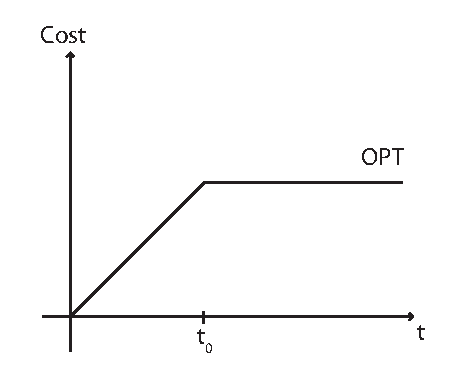
\includegraphics{Figures/Fig1}
	\caption{The optimal solution to the problem (cost in function of the time of the first request)} \label{fig1}
\end{figure}

It should be noted though that this algorithm is only theoritical~: it is not practical because it requires to know the value of $t_1$ to know what to do.

\paragraph{The best approximating deterministic algorithm}

Now a deterministic algorithm would have to decide a time $w$ at which it would shut down the hard drive and wait for the request if it's not arrived yet. For such an algorithm $A_w$, the cost graph is thus figure \ref{fig2} (there are two cases depending on whether $w$ is less or more than $y/x$).

\begin{figure}
	\centering
	\subfloat[Case when $w \leq y/x$]{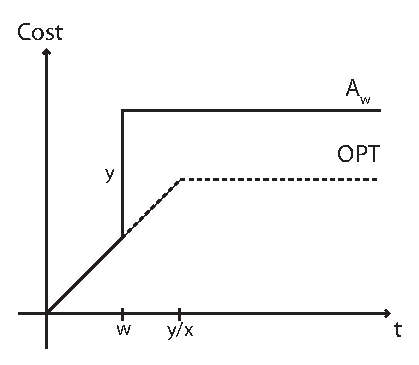
\includegraphics[width=6cm]{Figures/Fig2a}}
		\hspace{1cm}
	\subfloat[Case when $w \geq y/x$]{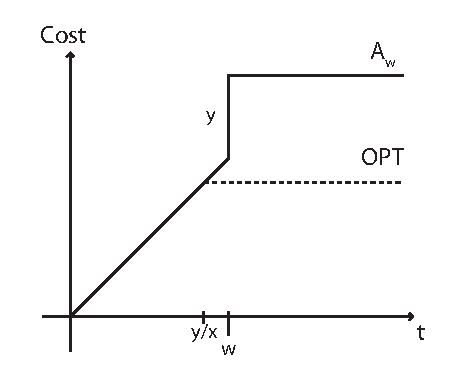
\includegraphics[width=6cm]{Figures/Fig2b}}
	\caption{The deterministic solution $A_w$ to the problem (optimal solution in strokes)} \label{fig2}
\end{figure}

\medskip

How good is such an algorithm compared to the optimal one~? We mesure that by calculating the approximation ratio~: $r = \max_t{\frac{cost(A_w, I_t)}{OPT_t}}$, where $cost(A_w, I_t)$ denotes the energy cost when using the algorithm $A_w$ if the request occurs at time $t$.

In the first case where $w \leq y/x$, we clearly have $r = \frac{x w + y}{x w} \geq 2$. Likewise, in the case where $w \geq y/x$, we have $r = \frac{x w + y}{y} \geq 2$.

This shows that any deterministic algorithm is at best a $2$-approximation of the optimal algorithm for solving the problem.

\smallskip

Moreover, by the previous expressions of $r$, we know that $A_{y/x}$ \emph{is} a $2$-approximation of the problem. So $A_{y/x}$ is the best approximating deterministic algorithm for our hard drive problem.

\medskip

If we go back to the real-life problem, this result means that without the use of randomness, one is doomed to use twice as much energy as optimally needed to run its hard drive.

Let's try to achieve a better result (on expectation) with a randomized algorithm.



\subsubsection{Using randomness to improve the algorithm}

\paragraph{Yao's Principle}

We will use Yao's principle on optimization problems, namely the following statement~:

\begin{theorem}
The cost of the best randomized algorithm on its worst instance is equal to the average cost of the best deterministic algorithm for the worst distribution of instances. More formally, 

\[ \min_p \max_q p A q = \max_q \min_p p A q\]

where $||p||_1=1, ||q||_1=1$ and $p,q \geq 0$
\end{theorem}

[See the notes on Yao's principle for more details about the notations and more insight on the meaning of this powerful principle.]


\paragraph{Application to the hard drive problem}

Here, we take as $A$ the following operator~: $C_{w,t} = \frac{cost(A_w, I_t)}{OPT_t}$, ie. the ratio on the instance $I_t$. The goal is to minimize this value, and Yao's principle provides a nice way to prove a lower bound on the competitive ratio of our problem.

Indeed, we have in particular that~:
\begin{equation} \label{eqn:yaomoitie}
\min_p \max_q p A q \quad \geq \quad \max_q \min_p p A q
\end{equation}

(which is actually the easy direction in Yao's principle). Following Yao's principle intuition, we can state that~: if $p$ is fixed, then $\max_q (pA)q$ can be seen as the worst case ratio of the randomized algorithm $pA$~; while when $q$ is fixed, $\min_p p(Aq)$ can be seen as the worst case ratio of the best deterministic algorithm on the distribution $q$.

Let's assume that we have found two distributions $p^\star$ and $q^\star$ such that $\max_q p^\star A q = \min_p p A q^\star$. Then by the inequality (\ref{eqn:yaomoitie}), it is clear that this value is actually the value $\min_p \max_q p A q = \max_q \min_p p A q$. And as the quantity $\max_q p^\star A q$ defines exactly the best randomized algorithm's competitive ratio, we have a lower bound on the best competitive ratio it is ever possible to achieve.

It is now time to actually find $p^\star$ and $q^\star$~: $p^\star$ provides the randomized algorithm, while the equality in (\ref{eqn:yaomoitie}) with the help of $q^\star$ proves that it is actually optimal.


\paragraph{$p^\star$ and $q^\star$}

Let us first simplify the notations to make computations easier. Without loss of generality, up to rescaling of time and cost, we can assume that $x=y=1$. We denote by $d$ the value of $w$ in this rescaled context. Then by definition, we have :

\begin{equation} \label{eq:eq1} \frac{cost(A_d,I_t)}{OPT_t} = \left\{\begin{array}{ll}
 \frac{d+1}{t}  & \text{ if }0 \leq d \leq t \leq 1 \\
 d+1 & \text{ if } 0 \leq d \leq t \text{ and } t >1 \\
 d & \text{ if } d >t>1 \\
 1 & \text{ otherwise } \end{array}\right. \end{equation}


This equation asks for two remarks.
\begin{itemize}
\item \textbf{First remark} : we can assume that $d \leq 1$ in the best deterministic algorithm (otherwise it would have been better to just shut down the hard drive to begin with).
\item \textbf{Second remark} : for $t >1$, the competitive ratio decreases, so we can assume that $t \leq 1$.
\end{itemize}

Now, looking at both these remarks and with some insight and some luck, let us guess the best randomized algorithm. The key is to think of an exponential distribution.

The "miracle" distribution is as follows. $d$ being a continuous value, the distribution is given by its density function : $p^\star(d) = \Pr_x(x \geq d)$

$$p^\star(d)= \left\{\begin{array}{ll} \frac{e^d}{e-1} & \text{if} \quad 0 \leq d \leq 1\\ 0 & \text{otherwise}\end{array}\right.$$

This is a density function since $\int_{\mathbb{R}} p^\star(d) d d = \int_0^1 \frac{e^d}{e-1}dd =1$.

Recall that the competitive ratio of a randomized algorithm is :

\[CR(A_{p^\star}) = \max_{t} \frac{ \mathbb{E}_{p^\star}(cost(A_{p^\star},I_t))}{OPT_t} \]


For a fixed $t$, this can be computed using equation (\ref{eq:eq1})~:

\begin{eqnarray*}
\frac{ \mathbb{E}_{p^\star}(cost(A_{p^\star},t))}{OPT_t}&=&\int_0^1 p^\star(d) CR(A_{d,t}) dd \\
&=& \int_0^t \frac{e^d}{e-1} \frac{d+1}{t}dd + \int_t^1 \frac{e^d}{e-1} 1 dd \\
&=& \frac{1}{e-1} ( \frac{1}{t} [e^t-1] + e-e^t + \frac{1}{t}\int_0^t de^d dd) \\
&=& \frac{e}{e-1}
\end{eqnarray*}

which is independent of $t$, and much less than 2 (about 1.4) ! This calculation provides us with a randomized algorithm of competitive ratio $\frac{e}{e-1}$.

\medskip

Now let us prove the lower bound. We need to find a distribution $q^\star$ such that no deterministic algorithm can beat this ratio, which will provide a lower bound using Yao's lemma as explained above.

Using again some insight and some luck, we propose the following miracle distribution~:

$$q^\star(t) = \left\{\begin{array}{ll} t \frac{e^{1-t}}{e-1} & \text{ if }  0\leq t <1 \\
0 & \text{ if } t >1\end{array}\right.$$

and $Pr(t=1) = \frac{1}{e-1}$.

Once again, this is a correct distribution since $\int_0^1 q^\star(t)dt + Pr(t=1)=\frac{e}{e-1}(-e^{-1} - e^{-1}+1)+\frac{1}{e-1}=\frac{-2+e+1}{e-1}=1$. 

To conclude, we just need to compute the average competitive ratio of any deterministic algorithm on this distribution, using equation (\ref{eq:eq1}) again :

\begin{eqnarray*}
E(\frac{cost(A_d,I_t)}{OPT_t}) &= &\int_0^d t \frac{e}{e-1}e^{-t}dt + \int_d^1 \frac{d+1}{t}t \frac{e}{e-1} e^{-t}dt + \frac{1}{e-1}(d+1)\\
&=& \frac{e}{e-1}(-de^{-d}-e^{-d}+1) + (d+1)\frac{e}{e-1}(e^{-1}-\frac{1}{e})\\
&=&\frac{e}{e-1}
\end{eqnarray*}

We conclude using Yao's Lemma that the randomized algorithm using the distribution $p^\star$ is optimal. This calculation is fairly tedious but otherwise the proof is simple, hence it makes a good example on how to prove lower bounds on randomized algorithms.

\bigskip

In the end, we found a (optimal) randomized algorithm which consumes on expectation only $40\%$ more energy than optimally necessary, instead of the $100\%$ we found in the deterministic case.






\newpage
\section{Randomized rounding}

Most optimization problems are NP-complete, and therefore cannot be solved directly
at low cost. As a solution, we can use a simplified version of the problem which
would be easier to solve (by, for instance, releasing constraints). But when
translating the optimum of the simplified problem back to the original setting, we
have no guarantee that the optimality is preserved. We can therefore wonder how far
this rounded optimum is from the actual optimum. Bounding this distance will enable
us to link the obtained optimum to the one of the first problem. We will focus in
this chapter on the Max-SAT problem.\\

\begin{center}
 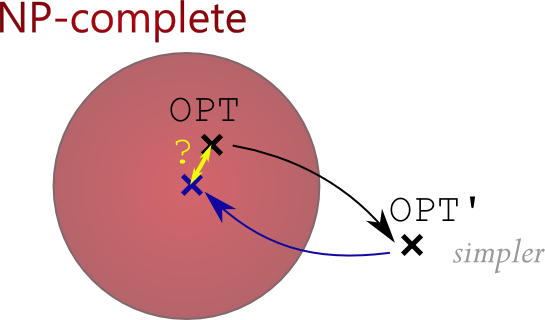
\includegraphics[width=0.6\textwidth]{Figures/img1}
\end{center}



%\subsection{Derandomizing MAX-SAT using Conditional Expectation}
\subsection{Approximation algorithms for Max-SAT}
Max-SAT is the typical problem in order to study results about approximations.\\

\textbf{Max-SAT}\\
Given a boolean formula $\phi$ on $x_1, \dots, x_n$ written in Conjunctive Normal
Form, $\displaystyle \phi = \bigwedge_{j=1}^m{C_j}$ where clauses $\displaystyle
C_j=\bigvee_{k=1}^{l_j}{L_k}$,
$L_k\in \{x_i, \neg x_i\}$, the problem is to compute the maximum number of clauses
an assignment on the $x_i$ can satisfy.\\

The SAT problem, which is NP-complete, is clearly a particular case where all the
clauses are satisfied: unless P=NP, there is no algorithm that can decide in polynomial time
whether Max-SAT = $m$ or not. The fact to distinguish between $(m-1)$ and $m$
satisfied clauses is therefore NP-complete. The PCP theorem enables to widen this
result: being able to distinguish between $(\frac{7}{8}+\epsilon)m$ and $m$
satisfied clauses would mean being able to solve any NP problem. That is why, $\forall\epsilon>0$, there
is no  $(\frac{7}{8}+\epsilon)$-approximation for this problem. Note
that the result also stands when all the clauses have length 2, but the constant
$\frac{7}{8}$ is specific to clauses of length 3.

\begin{center}
 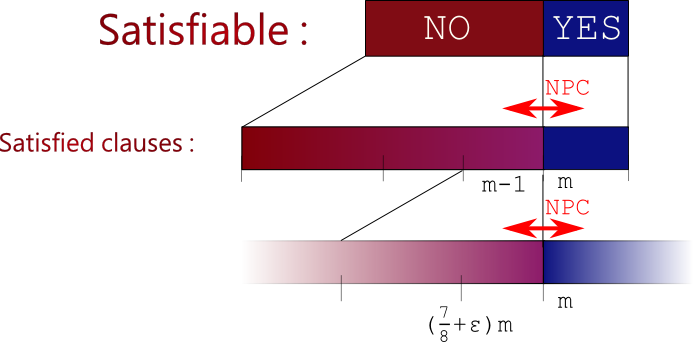
\includegraphics[width=0.6\textwidth]{Figures/img2}\\
\end{center}

Randomization does not seem to have a huge impact on such problems: the speedup is
limited, because most randomized algorithm have inspired deterministic equivalent
solutions. As a general rule, if there exists a very hard problem, we can use it to
generate pseudorandom strings, which we can then use to derandomize any randomized
algorithm, limiting the impact of randomization. In the other case, we can show that
the permanent is hard to compute. \\




%\subsubsection{Randomized algorithm}

Let us consider MAX-SAT has $m$ clauses with each clause $C_j$ having $l_j$ literals in it. Let the MAX-SAT
function be denoted by $\phi$. Let us assume the literal $x_i$ is $true$ in the original MAX-SAT $\phi$ gets transformed to  $\phi_i^0$ 
and similarly $\phi_i^1$ when we assume $x_i$ is false.

Let us consider an assignment on the $x_i$, and let $y_1, \dots, y_n$ and $Z_1, \dots,
Z_m$ be variables in $\{0,1\}$ such that:
\begin{align*} 
y_i &= \left\{ \begin{array}{l l}
    1 & \quad \text{if $x_i$ is true}\\
    0 & \quad \text{if $x_i$ is false}\\
\end{array} \right. \\   
Z_j &= \left\{ \begin{array}{l l}
    1 & \quad \text{if the clause $C_j$ is satisfied}\\
    0 & \quad \text{otherwise}\\
\end{array} \right.
\end{align*} 

We use the notation $L_j^+ = \{ i : x_i \in C_j \}$ and $L_j^- = \{ i | \bar{x_i} \in C_j \}$ where $C_j$ is a clause and $x_i$ is a literal.

\subsubsection{Algorithm 1 - Random Assignment + Derandomization}
%Random assignment should be the lower bound for the performance of any algorithm proposed because 
%it is the simplest possible way of solving a problem. 
%\begin{eqnarray}
%E(\mbox{cost(Algorithm 1)}) =  \sum_{j=1}^m E(z_j) = \sum_{j=1}^m Pr(z_j = 1) = \sum_{j=1}^m 1 - \frac{1}{2^{l_j}} \geq (1 - \frac{1}{2^{l_{min}}}).m \nonumber
%\end{eqnarray}
%where $l_{min} =$ size of the smallest clause in the MAX-SAT.

The easiest solution to this problem is to try random assignments.\\
Since a clause is satisfied if at least one of its $l$ literals is true, the
probability for a single clause to be satisfied by a random assignment (none of the
literals are true) is: 
\[\mathbb{P}=1-\left( \frac{1}{2} \right)^l\]
%For each such clause, we will introduce a random variable $Z_j$ which will be worth
%1 if the random assignment satisfies the clause $C_j$, or 0 otherwise.\\
Hence, the expected result of such a random algorithm, that is to say the expected
number $\mathbb{E}$ of satisfied clauses, is:
\[\mathbb{E} = \sum_{j=1}^{m}{\mathbb{E}[Z_j]} = \sum_{j=1}^{m}{1 \times \left(
1-\left( \frac{1}{2} \right)^l \right)} 
\geq m \times \left( 1-\left( \frac{1}{2} \right)^{l_{min}} \right)\]
By linearity of expectation and with $l_{min} = \min (l_j)$\\
If all the clauses have at least 3 literals, this last term is worth $\frac{7}{8}$:
$\mathbb{E} \geq \frac{7}{8} m$: it is therefore optimal. But this algorithm is very
bad if there exist a clause with a few number of literals (if there is a clause with
1 literal, we can only guarantee that half the clauses will be satisfied). This is
the case that needs improving.

	\paragraph{Derandomization}
Using cost of expectation of the algorithm in equation-\label{algo-1} we can derandomize this algorithm in the following way. Let us consider a literal $x_i$. 
\begin{eqnarray}
E(\mbox{cost(Algorithm1)}) & = & E(\mbox{cost(Algorithm1)} | y_i = 0) Pr(y_i = 0) \nonumber \\
                            & + &E(\mbox{cost(Algorithm1)} | y_i = 1) Pr(y_i = 1) \nonumber
\end{eqnarray}
which is using the average of the Expectation of the algorithm conditioned on literal $y_i$. Instead if we consider to assign a
value to $y_i$ a value which maximizes using the conditional expectation i.e. $\max_a E(\mbox{cost(Algorithm1)} | y_i = a)$
where $ a \in \{0,1\}$.

The expectations conditioned on variable $y_i$ can be calculated as  
\begin{eqnarray}
E(\mbox{cost(Algorithm1)} | y_i = 0) & = &\sum_{C_j \in \phi_i^0} ( 1 - \frac{1}{2^l_j}) \nonumber \\
E(\mbox{cost(Algorithm1)} | y_i = 1) & = &\sum_{C_j \in \phi_i^1} ( 1 - \frac{1}{2^l_j}) \nonumber
\end{eqnarray}
The above costs can be calculated deterministically in polynomial time. Hence we greedily assign $y_i$ the value that increases the expected cost of
the algorithm.


\subsubsection{Algorithm 2 - Linear Programming + Derandomization}

Max-SAT is equivalent to the following linear problem (with the previous definitions):

\begin{eqnarray}
MAXSAT(\phi) & = &\max \sum_{j=0}^m z_j \nonumber \\
&\forall Z_j,~Z_j \leq &\sum_{i \in L_j^+} y_i + \sum_{i \in L_j^-} (1 - y_i) \nonumber \\
&\forall j,~ z_j \in \{0, 1\} \nonumber \\
&\forall i,~  y_i \in \{0, 1\} \nonumber 
\end{eqnarray}

Unfortunately, we do not know any polynomial algorithm able to solve such a linear
problem. But, if we replace the conditions $y_i \in \{0,1\}$ and $z_j \in \{0,1\}$
by the conditions $y_i, z_j \in \mathbb{R}$ and $0 \le y_i, z_j \le 1$, this problem
can be solved in polynomial time (for example using the ellipsoid algorithm of
Khachiyan). Let $OPT$ be the maximum value for the original problem and $OPT_f$ be
the one for the problem with real variables (clearly $OPT_f \ge OPT$). Using this
technique, we can propose the following algorithm:


\begin{theorem}[{\bf An algorithm based on linear programming}]
~
\begin{enumerate}
\item Compute an optimal solution for the above problem with variables in $[0,1]$.
Let $y^*_1, \dots, y^*_n$, $z^*_1, \dots, z^*_m$ this solution.
\item Set $x_i = 1$ with probability $y^*_i$ (independently).\\
\end{enumerate}
The proposed algorithm is so a $(1 - \frac{1}{e})$-randomized approximation for
Max-SAT.
\end{theorem}

The expected number $\mathbb{E}$ of satisfied clauses, is:
\[ \mathbb{E} = \sum_{j=1}^{m}{\mathbb{E}[Z_j]} \]
(as in the previous subsection, we define $Z_j = 1$ if and only if the clause $C_j$ is
satisfied)

Without loss of generality, we can renumber the variables and replace $x_i$ by $\neg
x_i$ such that:
\[ C_1 = x_1 \vee \dots \vee x_l \]
where $l = l_1$.

Then:
\begin{align*}
\mathbb{P} (Z_1 = 1) &= 1 - \mathbb{P} \left( \bigcap_{i=1}^l \{ x_i = 0 \} \right) \\
&= 1- \prod_{i=1}^l \mathbb{P}(x_i = 0) \quad \text{by independence of the $x_i$} \\
&= 1 - \prod_{i=1}^l (1 - y^*_i)
\end{align*}

Since the logarithm function is concave: for all $a_1, \dots, a_l \in \mathbb{R^*_+}$:
\begin{align*}
\frac{1}{l} \sum_{i=1}^l \log a_i \; &\le \; \log \left( \sum_{i=1}^{l}
\frac{a_i}{l} \right) \\
\prod_{i=1}^l a_i \; &\le \; \left( \sum_{i=1}^{l} \frac{a_i}{l} \right) ^ l
\end{align*}

And so:
\[
\mathbb{P} (Z_1 = 1) \ge 1 - \left( \sum_{i=1}^{l} \frac{1 - y^*_i}{l} \right) ^
l = 1 - \left(1 - \sum_{i=1}^{l} \frac{y^*_i}{l} \right) ^ l 
\]

But we also have: $z^*_1 \le \sum_{i=1}^{l} y^*_i$ since the $y^*_i$ and the $z^*_j$
verify the constraint of the previous linear problem. Hence:
\begin{equation} \label{eq:probaZ1}
 \mathbb{P} (Z_1 = 1) \ge 1 - \left( 1 - \frac{z_1}{l} \right)^l
\end{equation}

Let $g : \left( \begin{array}{l c l}
    [0,1] & \rightarrow & \mathbb{R}\\
    x & \mapsto & 1- (1-\frac{z}{l})^l - (1-\frac{1}{e}) z
    \end{array} \right)$
    
If $l=1$, $g(z) = 1 \ge 0$. Otherwise $l \ge 2$ and:
\begin{align*}
g'(z) &= \left( 1 - \frac{z}{l} \right)^{l-1} - \left(1 - \frac{1}{e} \right) \\
g''(z) &= \frac{l-1}{l} \left( 1 - \frac{z}{l} \right)^{l-2} \ge 0
\end{align*}
$g$ is then concave and so its minimum is either $g(0) = 1$ or $g(1)$. And, since
the logarithm function is concave:
\begin{equation} \label{eq:classicIneq}
 \left(1 - \frac{1}{l}\right)^l = e^{l \log(1-\frac{1}{l})} \le e^{-\frac{l}{l}} =
\frac{1}{e} 
\end{equation}

This means $g(1) = 1- (1-\frac{1}{l})^l - (1-\frac{1}{e}) \ge 0$ and so $g(z) \ge 0$
for all $z \in [0,1]$.

Hence, according to equation~\eqref{eq:probaZ1}:
\[ \mathbb{P} (Z_1 = 1) \ge g(z^*_1) + \left( 1 + \frac{1}{e} \right) z^*_1 \ge
\left( 1 - \frac{1}{e} \right) z^*_1 \]

and:
\[ \mathbb{E} \ge \sum_{j=1}^m \left( 1 - \frac{1}{e} \right) z^*_j = \left( 1 -
\frac{1}{e} \right) OPT_f \ge \left( 1 - \frac{1}{e} \right) OPT \]

The proposed algorithm is so a $(1 - \frac{1}{e})$-randomized approximation for
Max-SAT. This is better than the first algorithm only for small clauses (when
$l_{min} = 1$, $1 - \frac{1}{e} \ge 1 - \frac{1}{2^{l_{min}}}$).

\paragraph{Derandomization}
We can derandomize this algorithm also similar to the derandomizing the above Algorithm-1 by calculating the conditional expectations and assigning the 
value which fetches maximum expected cost.
\begin{eqnarray}
E(\mbox{cost(Algorithm2)} | y_i = 0) & = &\sum_{C_j \in \phi_i^0} ( 1 - \prod_{i\in L_j^+}(1 - y_i^*) \prod_{i \in L_j^-} y_i^*) \nonumber \\
E(\mbox{cost(Algorithm2)} | y_i = 1) & = &\sum_{C_j \in \phi_i^1} ( 1 - \prod_{i\in L_j^+}(1 - y_i^*) \prod_{i \in L_j^-} y_i^*) \nonumber
\end{eqnarray}


\subsubsection{Combining both}

The first algorithm behaves better with clauses with a lot of literals whereas the
second one behaves better with clauses with few literals. Therefore it would be good
to combine this two algorithms.

An idea is to choose randomly the algorithm to run: run
the first one with probability $p$ and the second one with probability $1-p$ ($p$
will be fixed later).

In this case we have:
\[
\mathbb{E} = \sum_{j=1}^{m}{\mathbb{P}(Z_j = 1)}
\]
and:
\begin{align*}
\mathbb{P}(Z_j = 1) &\ge p \left( 1 - \frac{1}{2^{l_j}} \right) + (1-p) \left( 1 -
\left(1-\frac{1}{l_j}\right)^{l_j} \right) \\
&\ge 1 - p \frac{1}{2^{l_j+1}} - (1-p) \left(1-\frac{1}{l_j}\right)^{l_j} = p_j
\end{align*}

\begin{itemize}
\item if $l_j = 1$, $p_j = 1 - \frac{p}{2}$ and $p_j \ge \frac{3}{4}$ if $p \le
\frac{1}{2}$.
\item if $l_j = 2$, $p_j = 1 - \frac{p}{4} - \frac{1-p}{4} = \frac{3}{4}$.
\item if $l_j \ge 3$ and $p= \frac{1}{2}$:
\[ p_j = 1 - \frac{1}{2^{l+1}} - \frac{1}{2} \left( 1 - \frac{1}{l} \right)^l \ge 1
- \frac{1}{2^4} - \frac{1}{2}\frac{1}{e}  \approx 0.753 \ge \frac{3}{4}\]
(the first inequality comes from the equation~\eqref{eq:classicIneq}
page~\pageref{eq:classicIneq})
\end{itemize}

The goal is to maximize over $p$ the minimum over $l_j$ of $p_j$. Since if $l_j =
2$, $p_j = \frac{3}{4}$, necessarily this minimum over $l_j$ is greater or equal
than $\frac{3}{4}$. Furthermore with $p=\frac{1}{2}$, the result minimum is
$\frac{3}{4}$. So set $p=\frac{1}{2}$.

Therefore, this final algorithm is a $\frac{3}{4}$-random approximation of the Max-SAT
problem (which is better than the two other algorithms when $l_{min} = 1$).

But this could still be improved by running the two first algorithms and taking the
best result. The resulting algorithm will be at least a $\frac{3}{4}$-random
approximation of the Max-SAT problem for $l_{min} = 1$ and a $(1 -
\frac{1}{2^{l_{min}}})$-random approximation otherwise.

\newpage
\section{Sample and Guess}



\subsection{Self-correction of integer multiplication}
\paragraph{First version}

We have the program $A$ (seen as a matrix $N\times N$), and it is supposed to be such that $A(x,y)=xy\mod N$, for $(x,y)\in[0,N-1]^2$. There might be bugs in the matrix (i.e. pairs $(x,y)$ such that $A(x,y)\ne xy\mod N$), but $|\#bugs|\le10\%$ of the pairs. We cannot check the correctness, how can we fix that with randomness ?\\

We can use the following procedure that provides $xy\mod N$ with probability $\ge60\%$
\begin{itemize}
\item Draw 2 random numbers $(r,s)\in[0,N-1]^2$
\item Output $A(x+r,y+s)-A(r,y+s)-A(x+r,s)+A(r,s)$
\end{itemize}

If $A$ provides the good results for our requests, we get :\\
$(x+r)(y+s)-r(y+s)-(x+r)s+rs=xy+xs+ry+rs-ry-rs-xs-rs+rs=xy$.

The access of $A$ asked are uniformly random. To be convinced of that, we just need the following lemma :

\begin{lemma}
  If $G$ is a group and $U$ a uniform random variable over $G$, then $\forall g\in G$, $g+U$ is a uniform random variable over $G$.
\end{lemma}
\begin{proof}
$\forall y\in G$, $\mathbb{P}\{gU=y\}=\mathbb{P}\{U=g^{-1}y\}=\frac{1}{|G|}$.

\end{proof}

With that, the probability that each of the entry of A required is wrong is $\le 10\%$. It implies that the output value is not equal to $xy\mod N$ with probability $\le 40\%$. $\mathbb{P}\{Failure\}\le 40\%$. Because it works for any input, if we repeat this process and take the majority of the value, we can have a probability of success as close to 1 as we want. (We can also compare the result to $A(x,y)$ to improve the program.)\\




Multiplication is "random-self reductible". This problem has a good "worst case" to deal with.

\paragraph{Second version}

Imagine that you have a deterministic program $A(x,y)$ that given two integers $x, y \in \{0,...,N-1\}$ is supposed to output $xy \mod N$, but unfortunatelly, it might be buggy. Let us assume that it gives wrong answers on 10\% of the input pairs (we do not know which ones, of course). The algorithm is a black-box for us, so we cannot track down the bug in the program's code. Still, we have a way of fixing it by using randomness.

The crucial property is that multiplication in random self reducible, which means that if we know how to compute it on random instances, we know how to compute it on arbitrary instance. Let's see how it works.

We draw independently two random numbers, $r, s \in \{0,...,N-1\}$, and we output $A(x+r, y+s) - A(x+r, s) - A(r, y+s) + A(r,s)$. Note that all four of the input instances are random. Now, if there are no errors, the output is equal to $(x+r)(y+s) - (x+r)s - r(y+s) + rs = xy$, and the probability of error is less than 40\%. 
Why is it an improvement? Because we have reduced computing multiplication on an arbitrary instance (possibly a worst-case instance, where the deterministic algorithm $A$ always errs) to computing multiplication on random instances with non-zero probability of success (which we can even amplify).

Why are the instances random? We have the following easy lemma:

\begin{lemma} If $G$ is a group and $U$ a uniform random variable over $G$, then $\forall g \in G, \quad gU$ is a uniform random variable.\end{lemma}
\begin{proof} $\forall y \in G \quad \mathbb{P}\{gU = y\} = \mathbb{P}\{U=g^{-1}y\} = {1 \over |G|}$ \end{proof}



\subsection{Probabilistically Checkable Proofs (PCP)}

\subsubsection{Definitions of the class PCP$(r,q)$ and GAP-3SAT$_{1,c}$}
\begin{definition}
PCP$(r,q)$=$\left\{
\begin{array}{r l}
L| & \exists\text{bPTTM V  st :}\\
 & \text{1 : V uses }\theta(r)\text{ random bits}\\
 & \text{2 : }V(x,y)\text{ probes only }\theta(q)\text{ bits of y}\\
 & \text{3 : if x}\in L,\exists \text{ y st }\mathbb{P}\{V(x,y)=1\}=1\\
 & \text{4 : if x}\not\in L,\forall \text{ y }\mathbb{P}\{V(x,y)=1\}\le\frac{1}{2}\\
\end{array}
\right\}$
\end{definition}

\begin{definition}
SAT=$\left\{
\begin{array}{r l}
\varphi(x)=\bigwedge\limits_{i=j}^mC_j(x)| & \exists \text{x st }\forall j,C_j(x)=1\\
\end{array}
\right\}$

$\varphi=\bigwedge\limits_{i=j}^mC_j\in$SAT iff $\exists x$ satisfying the $m$ clauses.

$\varphi\not\in$SAT iff $\forall x$, $x$ satisfies at most $m-1$ clauses of $\phi$.
\end{definition}

In that way, there is a gap between the number of accepted clause by $\varphi$ depending on weather $\varphi$ is in SAT or not.

The gap is :
\begin{itemize}
\item $\ge m$ satisfiable clauses at the same time if $\varphi\in$L.
\item $\le m-1$ satisfiable clauses at the same time if $\varphi\not\in$L.
\end{itemize}

We will now amplify this gap, asking that at most $cm$, with $c<1$, clauses are satisfiable at the same time if $\varphi$ is not totally satisfiable.

\begin{definition}
GAP-3SAT$_{1,c}$ is such that :
\begin{itemize}
\item $\varphi\in$GAP-3SAT$_{1,c}$ if $\varphi$ is satisfiable
\item $\varphi\not\in$GAP-3SAT$_{1,c}$ if at most $cn$ clauses of $\varphi$ can be simultaneously satisfied
\end{itemize}
\end{definition}

\subsubsection{PCP and NP theorem}

We want to prove the theorem :

\begin{theorem}
NP=PCP$(\log n,1)$
\end{theorem}

\paragraph{First version}
For that, we will first prove that PCP$(log\,n,\,1)\,\subseteq\,$NP.

Indeed, the verifier choses $r=O(log\,n)$ bits randomly, which means $2^r=Poly(n)$ random choices possible. Thus, the verifier can check all random strings in polynomial time to find whether a word is in the langage or not.
\\

In order to study the property NP$\,\subseteq\,$PCP$(log\,n,\,1)$, we will use the introduced problem GAP-3SAT$_{1,c}$. We have the following property :
\begin{prop}
NP$ \, \subseteq \, $PCP$(log \, n, \, 1) \, \Longleftrightarrow \, \exists $ $c < 1, \, $GAP-3SAT$_{1,c}$ is NP-hard
\end{prop}
This proposition is equivalent to :\\
$(\exists c <1,\,\forall \varepsilon > 0)\,\exists\,a\,(c+\varepsilon)-$approximation for MaxSAT $\Longrightarrow $P=NP

\subsubsection{Proof $\Longleftarrow$}

In the proposition 1, the direction $\Longleftarrow$ is the easiest to prove.

Indeed, if GAP-3SAT$_{1,c}$ is a NP-hard problem, then we have a polynomial time reduction. For any language $L \in $NP we have the function $x\mapsto \varphi_{x}$ so that :
\begin{itemize}
\item if $x \in L,\,\varphi_{x}\in $SAT
\item if $x \notin L$, at most $cn$ clauses of $\varphi_{x}$ are satisfied simultaneously
\end{itemize}
$ $

Then, we will create a PCP-verifier which will be $V(x,y)$ where $y=y_{1}...y_{l}$ is the value of the variables of $\varphi_{x}$. The verifier will :
\begin{enumerate}
\item Draw a random clause of $\varphi_{x}$, $C_{j}$
\item Output $C_{j}(y)$
\end{enumerate}
$ $

Indeed, if $x \in L$, $\varphi_{x}$ is satisfiable, so $\exists y$ such that any clause is satisfiable. Then, whatever clause I chose, $C_{j}(y)=1$. If $x \notin L$, at most $cn$ clauses of $\varphi_{x}$ can be satisfied simultaneously so whatever $y$ I chose, there is a constant probability that $C_{j}(y)=0$. $V$ is well defined as a PCP-verifier.

We can check that the parameters are correct, that $L \in $PCP$(log\, n, 1)$ : The clause chosen randomly among a number of clauses polynomial in the size of $x$, so we need $O(log\,|x|)=O(log\,n)$ bits to chose the clause. Then, we use only the value of only $3=O(1)$ variables, in order to calculate the value of the clause. $V$ is a $(log\,n,\,3)$-verifier.

\subsubsection{Proof $\Longrightarrow$}
In the opposite way, we suppose NP$\,\subseteq\,$PCP$(log\,n,\,1)$.

Then, take $L \in NP$ and let $V$ be its $PCP$-verifier. $V$ uses $r=\theta (log\,n)$ random bits, asks for the value of $q=\theta (1)$ positions in y and outputs 0 or 1 such that :
\begin{itemize}
\item If $x \in L,\, \exists y,\, \mathbb{P}{V(x,y)=1}<1$
\item If $x \notin L,\, \forall y,\, \mathbb{P}{V(x,y)=0}>1/2$
\end{itemize}
$ $

For a random string $r$ and $q$ positions $y_{1},...,\,y_{q}$ in $y$, we definition $f_{r}(y_{1},...,\,y_{q})$ is the output of $V$ for such values. Thus, $f_{r}(y_{1},...,\,y_{q})$ is a $SAT$ formula of $2^q$ clauses, so it is a 3SAT formula of $(q-2)2^q=\theta(1)$. Then we have :
\begin{itemize}
\item If $x \in L,\, \exists y,\, \forall r,\,f_{r}(y_{1},...,\,y_{q})=1$
\item If $x \notin L,\, \forall y,\, \#\lbrace r|f_{r}(y_{1},...,\,y_{q})=1 \rbrace \leq \dfrac{1}{2} 2^r$
\end{itemize}
$ $

Now, let definition $\varphi_{x}=\bigwedge_{r}f_{r}(y)$. This formula can be computed in polynomial time, because there is a polynomial number of random string. This formula is of length $2^r(q-2)2^q$. Finally, we can choose $c=1-\dfrac{1}{q2^q}$. Any NP-problem can be reduce to GAP-3SAT$_{1,c}$, which proves the property.


\paragraph{Second version}

Less formally, this means that there are proofs for instances of the problems in the class NP that can be efficiently verified by a probabilistic machine that reads just a constant number of bits of the proof. 

It is easy to show that $NP \supseteq PCP(\log n, 1)$ -- we nondeterministically guess the PCP proof (it has polynomial length) and then check every random string (there is a polynomial number of them). The other inclusion is much harder.
\\

We will show that this theorem is equivalent to the existence of problems that cannot be approximated up to some constant factor $c$ unless P=NP.

Remember the definitions seen above. We now want to prove that the nontrivial inclusion in the PCP theorem is equivalent to the fact that for some $c<1$ GAPSAT$_{1,c}$ is NP-hard.
\\

{\bf If GAPSAT$_{1,c}$ is NP-hard, then $NP \subseteq PCP(\log n, 1)$.} Let $L$ be a language in NP. We want to create a PCP proof for $L$, given a reduction from $L$ to GAPSAT$_{1,c}$ that for every instance $x$ of $L$ creates a 3CNF formula $\varphi_x$. The PCP verifier $V$ expects the proof $y$ to be the satisfying assignment for $\varphi_x$. It then draws a random clause $\gamma$ and checks the values assigned to the three variables of $\gamma$ by the assignment $y$ (it needs to check only three bits of $y$) and accepts if and only if the clause is satisfied. Note that in the positive case it will always accept, and in the negative one it will accept with probability at most $c$ (with probability at most $c$ it will draw a clause satisfied by the assignment). We can amplify this probability gap by repeating the trial, given that $c$ is a constant less than 1.
\\

{\bf If $NP \subseteq PCP(\log n, 1)$, then GAPSAT$_{1,c}$ is NP-hard.} Take $L$ in NP and let $V$ be its $PCP(\log n, 1)$ verifier. Let $y = y_1 y_2 ... y_n$ be the proposed proof. For every random string $r$ we can create a formula $\varphi_r(y_{i_1}, y_{i_1}, ..., y_{i_q})$ over the boolean variables $y_1, y_2, ..., y_n$ and using at most a constant number $q$ of these variables, describing the output of the verifier $V$ given the string $r$ and a proof consistent with $y$ on the bits that $V$ queries. Note that such a formula is a disjunction of at most $2^q$ clauses describing the assignments to the proof bits that make $V$ accept. We can easily transform this formula to an analogous CNF formula with the same number of clauses (every clause says, informally, ``I am not this particular input that makes the verifier reject''). We can make a conjunction of such formulas for every $r$ (there is a polynomial number of them) creating a formula $\rho$ and use this formula as an input to GAPSAT. For the yes-instances of $L$ the verifier always accepts, so for every $r$ the formula $\varphi_r(y_{i_1}, y_{i_1}, ..., y_{i_q})$ has all clauses satisfied, which makes the whole formula $\rho$ satisfied. For the no-instances of $L$ the verifier rejects for at least half of the random strings, so the formulas assigned to these strings have at least one clause not satisfied, which creates the desired gap.


\newpage
%\usepackage{pst-all}



\subsection{One of the main step of the PCP theorem: $\NP \subseteq
\PCP(\mathrm{poly}(n),1)$}


\subsubsection{Introduction}
The goal of this lecture is to prove the following theorem
\begin{theorem}\label{theorem1}
$\NP \subseteq
\PCP(\mathrm{poly}(n),1)$
\end{theorem}

Although it is weaker than the PCP theorem it is one the main step of its proof.
We will use the following proposition:
\begin{prop}
The PCP class is stable under polynomial reduction. Formally:
\begin{displaymath}
(L\leq_P L' \quad\mathrm{and}\quad L'\in \PCP(\mathrm{poly}(n),1) \implies L\in
\PCP(\mathrm{poly}(n),1)
\end{displaymath}
\end{prop}

\begin{proof}
Let $M$ be a polynomial-time Turing machine transforming instances of $L$ in
instances of $L'$. Let $V$ be a polynomial-time verifier (with random access)
for the language $L'$:
\begin{displaymath}
L' = \{ x: \exists y, V(x,y) = 1 \}
\end{displaymath}
Then $(x,y)\mapsto V(M(x),y)$ is a polynomial-time verifier for the language
$L$. 
\end{proof}

Thus, if we prove for a single NP-complete problem that it is also in
$\PCP$, then all the problems that are polytime reducible to
it (that is, all the NP problems) will also be in $\PCP(\mathrm{poly}(n),1)$.
Here we will study the problem \textsf{QUADEQ}.

\begin{encadre}{\textwidth}
\begin{center}
\textbf{\textsf{QUADEQ} Problem}
\end{center}

\textbf{Input:} $n\in\mathbf{N}^*$, $m\in\mathbf{N}^*$, a set of $m$ quadratic
multivariate equations over $n$ variables: $x_1,\ldots,x_n$.

\textbf{Output:} Is it possible to find an assignment of the variables in
$(\mathbf{Z}/2\mathbf{Z})^n$ satisfying the set of equations?
\end{encadre}

\begin{example}
\textbf{Input:} $n=5$, $m=3$
\begin{displaymath}
\left\{\begin{array}{rl}
x_1x_2 + x_2x_3 + x_4x_1 & = 1\\
x_1x_3 + x_2x_4 & = 0\\
x_1x_3 + x_4x_5 + x_1x_2 & = 1        
\end{array}\right.
\end{displaymath}

\textbf{Ouput:} The set of equations is satisfiable. For example, $x_1 = x_2 =
  \ldots = x_5 = 1$ is a valid assignment.
\end{example}

In the next sections we will prove that \textsf{QUADED} is NP-complete and then
we will construct a $\PCP(n^2,1)$ verifier.

\subsubsection{NP-completeness of \textsf{QUADEQ}}

The proof is straightforward. First, we prove that \textsf{QUADEQ} is in
NP, then we prove that it is NP-hard by reducing \textsf{3-SAT} to it.

\paragraph{$\textsf{QUADEQ}\in\NP$:} It is easy to build a polynomial-time
verifier for \textsf{QUADEQ}: given an assignment of the variables
$(x_1,\ldots,x_n)$, the verifier just checks whether this assignment is valid
or not.

\paragraph{Reduction from \textsf{3-SAT} to \textsf{QUADEQ}:} Given a boolean
formula in 3-CNF we first build a boolean circuit which only contains
\textsf{NOT}, \textsf{AND} and \textsf{OR} gates. It is thus a binary tree where
the nodes are logical gates and where the leaves are the literals of the
boolean formula. This tree can be built by induction on the number of clauses:

\begin{itemize}
 \item Given a clause containing 3 literals: $(\lnot)? x \lor(\lnot)?
y\lor(\lnot)?z$ (here the question marks indicate that the \emph{not} operator
might or might not be there), we build the following circuit:

\begin{figure}[h]
\begin{center}
\pstree[treemode=U,levelsep = 1cm]{\TCircle{$\lor$}}{
\pstree{\TCircle{$\lor$}}{
  \pstree[nodesepB=5pt]{\TCircle{$?$}}{\Tr{$x$}}
  \pstree[nodesepB=5pt]{\TCircle{$?$}}{\Tr{$y$}}
}
\pstree[nodesepB=5pt]{\TCircle{$?$}}{\skiplevel{\Tr{$z$}}}
}
\end{center}
\end{figure}

Where the question mark is a $\textsf{NOT}$ gate if there is a $\lnot$
operator in the clause.

\item Suppose that we are given a formula with $(n+1)$ clauses. We first build
by induction a tree for the $n$ first clauses : $T_1$. Then we build a
tree $T_2$ for the last clause as explained in the previous step. Then the tree
for the whole formula will be:
\newpage
\begin{figure}[h]
\begin{center}
\pstree[treemode=U,levelsep = 1cm, nodesepB=5pt]{\TCircle{$\land$}}{
  \Tr{$T_1$}
  \Tr{$T_2$}
}
\end{center}
\end{figure}

It is easy to see that the size of the tree is linear in the size of the
formula.
\end{itemize}

Then we build a set of equations simulating the computation of the boolean
value of the formula. This computation is done from the literals (i.e. the
leaves) to the root: 

\begin{enumerate}
\item Attach a variable to each node and leaf of the tree.
\item Build the set of equations by induction (on the depth of the tree) using
the following rules:
\begin{itemize}
 \item For a not gate:
\begin{figure}[h]
\begin{center}
\pstree[treemode=U,levelsep = 1cm]{\TCircle{$\lnot$}~{$u_1$}}{
\TCircle{}~[tnpos=l]{$u_2$}
}
\end{center}
\end{figure}

Add the equation: $u_1 = 1+u_2$
\item For a two-wired gate:
\begin{figure}[!h]
\begin{center}
\pstree[treemode=U,levelsep = 1cm]{\TCircle{?}~{$u_1$}}{
\TCircle{}~[tnpos=l]{$u_2$}
\TCircle{}~[tnpos=r]{$u_3$}
}
\end{center}
\end{figure}

If it is a \textsf{AND} gate, add the equation: $u_1$ = $u_2u_3$. If it is a
\textsf{OR} gate, add the equation: $u_1 = 1 - (1-u_2)(1-u_3)$.
\end{itemize}
\end{enumerate}

Let $(u_1,\ldots,u_n)$ be a solution to this set of equations where:
\begin{itemize}
 \item $u_n$ is the variable attached to the root node.
\item $(u_1,\ldots,u_r)$ are the variables attached to the leaves (i.e the
literals of the inital formula).
\end{itemize}
Then $u_n$ is exactly the boolean value of the inital formula for the
assignment $(u_1,\ldots,u_r)$ of the literals. Thus we add a final equation to
this set of equation: $u_n=1$. We obtain a system of quadratic equations
such that: \emph{the system has a solution if and only if there
exists an assignment of the literals satisfying the boolean formula}. This
gives us a reduction from \textsf{3-SAT} to \textsf{QUADEQ} and the NP-hardness
of \textsf{QUADEQ}.

\newpage
\subsubsection{A $\PCP(n^2,1)$ verifier for \textsf{QUADEQ}}

In this subsubsection, we describe a PCP verifier for \textsf{QUADEQ}. 

\paragraph{Notations:} First we can notice that in $\mathbf{Z}/2\mathbf{Z}$ we
have $x^2=x$. Hence, we can assume that all equations only have terms of degree
2. For example, an equation of the form $xy + x =1 $ can be replaced by the
equation $xy + x^2=1$.

An instance of a \textsf{QUADEQ} over the variables $x_1,x_2,\ldots,x_n$ can be
written $AX=b$ where:
\begin{itemize}
\item $A$ is a $m \times n^2$ matrix, $(A_{k,( i, j)})$, where
$k\in\{1,\ldots,m\}$ and $(i,j)\in\{1,\ldots,n\}^2$: $ A_{k,( i, j)}$ is the
coefficient of $x_ix_j$ in the $k^{th}$ equation.
\item  $b = (b_k)_{1\leq k\leq m}\in\{0,1\}^m$: $b_k$
is the constant term of the $k^{th}$ equation.
\item $X_{( i, j)}=x_{i}x_{j}=x\otimes x$ where $(i,j)\in\{1,\ldots,n\}^2$.
\end{itemize}

$X$ will not be computed by the verifier because this would require to probe
more than a constant number of positions in $x$. But the proof can be
exponentially large, so the proof will also contain $X$ and the verifier will
verify that $X$ is indeed related to $x$: $X=x\otimes x$.

Still, it is not to possible to verify that $X=x\otimes x$ with a constant
number of probes to $x$. The proof will give an encoding $X$ and $x$ more
suited to such computations: the \emph{Walsh-Hadamard} encoding.

\paragraph{Walsh-Hadamard encoding:} Let $x\in\{0,1\}^n$ the vector we want to
encode, let us define:
\begin{displaymath}
\begin{array}{rrl}
f_x:&\{0,1\}^n&\longrightarrow\{0,1\}\\
&r&\longrightarrow{}^tr\cdot x
\end{array}
\end{displaymath}
Then the encoding of $x$ is a table of size $2^n$: the truth table of the
linear function $f_x$. From $f_x$ we can recover $x$ by $x_i=f(e_i)$ where $e_i$
is the $i^{th}$ standard base vector ($i^{th}$ position equal to 1).

\paragraph{} The PCP verifier expects the proof to be:
\begin{itemize}
\item the table of a linear function $f:\{0,1\}^n\rightarrow\{0,1\}$: the
Walsh-Hadamard encoding of $x$, a valid assignment for the variables. This
table has size $n$.
\item the table of a linear function $g:\{0,1\}^{n^2}\rightarrow\{0,1\}$: the
Walsh-Hadamard encoding of $X$, such that $X=x\otimes x$. This table has size
$n^2$.
\end{itemize}

\begin{figure}[h]
\begin{center}
\begin{pspicture}(0,-0.5)(10,1)
\psframe(0,0)(5,0.6)
\psframe(4.95,0)(10,0.6)
\pcline[arrows=<->](0,-0.3)(5,-0.3)
\ncput*{$2^n$ bits}
\pcline[arrows=<->](5,-0.3)(10,-0.3)
\ncput*{$2^{n^2}$ bits}
\rput(2.5,0.3){$f:r\mapsto {}^tr\cdot x$}
\rput(7.5,0.3){$g:s\mapsto {}^ts\cdot (x\otimes x)$}
\end{pspicture}
\caption{Structure of the proof given to the PCP verifier}
\end{center}
\end{figure}

\newpage

The verifier works in three steps:
\begin{enumerate}
\item Check that $f$ and $g$ are linear: $x^f$ (resp. $X^g$) will denote the
vector encoded by $f$ (resp. $g$). 
\item Check that $X^g = x^f\otimes x^f$.
\item Check that $AX^g = b$.
\end{enumerate}

 
\paragraph{Check that $f$ and $g$ are linear functions}
We use linearity testing to check with $O(1)$ probes that $f$ and $g$ are
$0.999$ close to some linear functions $\tilde{f}$ and  $\tilde{g}$. If $f$ and
$g$ are indeed linear, this test is passed with probability $1$.

If none of $f, g$ is 0.999-close to a linear function, then the proof is
rejected with high probability. Therefore  we can assume for the rest that there
exist two linear functions $\tilde{f}$ and $\tilde{g}$ respectively 0,999-close
to $f$ and $g$.

By using linear decoding, we can also assume that the verifier is able to query
the value of $\tilde{f}$ and $\tilde{g}$ at any point with probability at least
$0.998=2 \times 0.999 -1$.

\paragraph{Check that $X^g = x^f\otimes x^f$}

The verifier does the following: 
\begin{itemize}
\item Choose two vectors $r$ and $r'$ in $\{0,1\}^n$ independently and
uniformly at random
\item Verify that $g(r\otimes r') = f(r)f(r')$ 
\end{itemize}
This test only requires two probes to the proof (a probe to the proof is
simply a query to one value of $f$ or one value of $g$).

Let us first rewrite the two terms of the test:
\begin{equation}\label{f}
f(r)f(r') = \left({}^tr\cdot x^f\right)\left({}^tr'\cdot x^f\right) 
= \left(\sum_{i=1}^n r_ix^f_i\right) \left(\sum_{j=1}^n r'_jx^f_j\right)
= \sum_{(i,j)} r_ir'_jx^f_ix^f_j
\end{equation}
\begin{equation}\label{g}
g(r\otimes r') = {}^t(r\otimes r')\cdot X^g=\sum_{(i,j)}r_ir'_jX^g_{(i,j)}
\end{equation}

\paragraph{Completeness of the test:} Assume that the proof is what we expect it
to be: the encodings of $X^g$ and $x^f$ such that $X^g = x^f\otimes x^f$. Then
we can rewrite~\eqref{g}:
\begin{displaymath}
g(r\otimes r') = \sum_{(i,j)}r_ir'_jx^f_ix^f_j = f(r)f(r')
\end{displaymath}
So if the proof is valid, the test will pass with probability 1.

\paragraph{Probability of failure:} Let us now assume that $X^g\neq x^f\otimes
x^f$, then we want to estimate the probability that the test will reject the
proof:
\begin{displaymath}
\prob{g(r\otimes r')\neq f(r)f(r')}
\end{displaymath}
Let us write, for any fixed $r'\in\{0,1\}^n$:
\begin{displaymath}
\Phi _{r'}:r\mapsto f(r)f(r') 
\end{displaymath}
\begin{displaymath}
\Psi _{r'}:r\mapsto g(r \otimes r')
\end{displaymath}
Then we have:
\begin{equation}\label{main}
\begin{split}
\prob{g(r\otimes r')\neq f(r)f(r')}
&= \prob{\Psi_{r'}(r)\neq\Phi_{r'}(r)}\\
&\geq \prob{\Psi_{r'}(r)\neq\Phi_{r'}(r)|\Psi_{r'}\neq\Phi_{r'}}
\prob{\Psi_{r'}\neq\Phi_{r'}}
\end{split}
\end{equation}

It is easy to see in \eqref{f} and \eqref{g} that $\Psi_{r'}$ and $\Phi_{r'}$
are linear. Hence, by using the fact two different linear functions differ on
at least half of their inputs:
\begin{equation}\label{first}
\prob{\Psi_{r'}(r)\neq\Phi_{r'}(r)|\Psi_{r'}\neq\Phi_{r'}} \geq \frac{1}{2}
\end{equation}

It remains to estimate $\prob{\Psi_{r'}\neq\Phi_{r'}}$. By using \eqref{f} and
\eqref{g}, we can rewrite:
\begin{displaymath}
\Phi_{r'}:r\mapsto{}^tr\cdot \big(x^ff(r')\big)
\end{displaymath}
\begin{displaymath}
\Psi_{r'}:r\mapsto{}^tr\cdot X_{r'}\quad\mathrm{with}\quad
X_{r'} = \left(\sum_{j=1}^n r'_jX^g_{(i,j)}\right)_{1\leq i\leq n}
\end{displaymath}
Hence, $\Psi_{r'}\neq\Phi_{r'}\Leftrightarrow\big(x^ff(r')\big)\neq X_{r'}$.
But the functions $r'\mapsto\big(x^ff(r')\big)$ and $r'\mapsto X_{r'}$ are also
linear, and if $X^g\neq x^f\otimes x^f$ then they are different and then differ
on at least half of their inputs. So:
\begin{equation}\label{second}
\prob{\Psi_{r'}\neq\Phi_{r'}}
=\prob{x^ff(r')\neq X_{r'}}
\geq\frac{1}{2}
\end{equation}

Plugging \eqref{first} and \eqref{second} into \eqref{main}, we get:
\begin{displaymath}
\prob{g(r\otimes r')\neq f(r)f(r')}\geq\frac{1}{2}\times\frac{1}{2}=\frac{1}{4}
\end{displaymath}
Then, at this step, the verifier will reject an invalid proof with probability
at least $1/4$.


\paragraph{Satisfiability: verify that $AX^g = b$}
We will assume here that the first two steps have passed: the functions
encoded in the proof are linear and encodes two vectors $x^f$ and $X^g$ such
that $X^g = x^f\otimes x^f$. It remains to verify that $x^f$ is a valid
assignment, i.e:
\begin{displaymath}
\forall k\in\{1,\ldots,m\},\;\sum_{(i,j)} A_{k,(i,j)}x^f_ix^f_j=b_k
\end{displaymath}
Note that $x^f_ix^f_j= X^g_{(i,j)}$ so this can be rewritten as:
\begin{displaymath}
\forall k\in\{1,\ldots,m\},\; {}^tA_k\cdot X^g = b_k
\end{displaymath}
And using the definition of $X^g$ (the vector encoded by $g$):
\begin{displaymath}
\forall k\in\{1,\ldots,m\},\; g(A_k) = b_k
\end{displaymath}
The problem is that the verifier cannot verify all these equations because it
would require more than a constant number of probes to $g$. So it will only
verify a random linear combination of the equations with the following
procedure:
\begin{itemize}
\item pick a vector $r\in\{0,1\}^m$ uniformly at random.
\item compute vector $A_r = \left(\sum_{k=1}^m r_kA_{k,(i,j)}\right)_{(i,j)}$
with $(i,j)\in\{1,\ldots,n\}^2$.
\item verify that $g(A_r) = {}^tr\cdot b$.
\end{itemize}

First remark that:
\begin{equation}\label{end}
\begin{split}
g(A_r) =
{}^tA_r\cdot X^g &= \sum_{(i,j)}\sum_{k=1}^m r_kA_{k,(i,j)}X^g_{(i,j)}\\
&= \sum_{k=1}^m r_k \sum_{(i,j)}A_{k,(i,j)}X^g_{(i,j)}\\
&= \sum_{k=1}^m r_k {}^tA_k\cdot X^g = {}^tr\cdot (AX^g)
\end{split}
\end{equation}
So probing the value of $g$ on vector $A_r$ is indeed equivalent to compute the
linear combination given by the random vector $r$ of the left part of the
system. The test then simply compares this linear combination to the same
linear combination of the right part of the system.

\paragraph{Completeness of the test:} Assume that $AX^g = b$, then for all $k$
in $\{1,\ldots,m\}$ we have ${}^tA_k\cdot X^g = b_k$, and plugging into
\eqref{end}
we get:
\begin{displaymath}
g(A_r) = \sum_{k=1}^m r_kb_k = {}^tr\cdot b
\end{displaymath}
Then if the proof is correct, the test will pass with probability 1.

\paragraph{Probability of failure:} Now assume that $AX^g \neq b$, then the two
functions $r\mapsto g(A_r)$ and $r\mapsto {}^tr\cdot b$ are linear and
different, so they differ on at least half of their inputs:
\begin{displaymath}
\prob{g(A_r)\neq {}^tr\cdot b} \geq \frac{1}{2}
\end{displaymath}
So in this case the verifier will reject the proof with probablility at least
$1/2$.
\newpage
To the sum up, we have built a $\PCP(n^2,1)$  verifier because :
\begin{itemize}
\item If the system is satisfiable, then there exists a proof that is accepted
with probability one and if the system is not satisfiable, any proof will be
rejected with a constant probability.
\item The verifier only makes $O(1)$ probes to the proof (each step consists in
probing a small number of random places in the proof and doing some computation
with them).
\item The verifier uses $O(n^2)$ random bits : indeed, it only needs to ask
random indexes in the proof table wich is $2^n+2^{n^2}$ big. So we need random
numbers between $1$ and $2^n+2^{n^2}$, wich only requires $O(n^2)$ bits.
\end{itemize}

Using this verifier and the fact that \textsf{QUADEQ} is also in NP, we have
finally prooved the theorem~\ref{theorem1}.




\newpage


\subsection{Constant time approximation}

We introduce a technique to transform approximations algorithms
into constant time algorithms that approximate the size of the optimal solution. 
In our case, we expose the technique for the approximating of the size 
of a maximal matching in some graph.


\subsubsection{A constant time algorithm}

In this paper, we shall denote our graphs $G$ as a couple of set $(V,E)$, whose first
component enumerates all vertices and the second component gives all edges. Besides,
we shall use the symbol $n$ to denote the cardinality of $V$ and we shall consider 
that the $G$'s degree is bounded by $d$.

\begin{definition}
Let $G = (V,E)$ be a graph, a \emph{matching} $M$ in $G$ is a set of pairwise non-adjacent
edges; that is, no two edges share a common vertex. A \emph{maximal matching} is a matching $M$
of a graph $G$ with the property that if any edge not in $M$ is added to $M$, then it is no longer a matching.
\end{definition}

\begin{remark}
Do not mistake maximal matchings with \emph{maximum matchings}, which are matchings containing the largest possible number of edges.
\end{remark}

\tikzstyle{vertex}=[circle,fill=black!25,minimum size=20pt,inner sep=0pt]
\tikzstyle{selected vertex} = [vertex, fill=red!24]
\tikzstyle{edge} = [draw,thick,-]
\tikzstyle{weight} = [font=\small]
\tikzstyle{selected edge} = [draw,line width=5pt,-,red!50]


\begin{figure}[h]
\centering
\subfloat[A matching non maximal.]
{
\begin{tikzpicture}[scale=1.3]
    \foreach \pos/\name in {{(0,2)/a}, {(2,1)/b}, {(4,1)/c},
                            {(0,0)/d}, {(3,0)/e}, {(2,-1)/f}, {(4,-1)/g}}
        \node[vertex] (\name) at \pos {$\name$};
	\path[selected edge] (d.center) -- (b.center);
%	\path[selected edge] (f.center) -- (e.center);
    \foreach \source/ \dest  in {b/a, c/b, d/a, d/b, e/b, e/c, e/d, f/d, f/e, g/e, g/f}
        \path[edge] (\source) -- (\dest);
    \foreach \vertex / \fr in {d/1,a/2,f/3,b/4,e/5,c/6,g/7}
        \path node[selected vertex] at (\vertex) {$\vertex$};
\end{tikzpicture}
}
\subfloat[A maximal matching non maximum.]
{
\begin{tikzpicture}[scale=1.3]
    \foreach \pos/\name in {{(0,2)/a}, {(2,1)/b}, {(4,1)/c},
                            {(0,0)/d}, {(3,0)/e}, {(2,-1)/f}, {(4,-1)/g}}
        \node[vertex] (\name) at \pos {$\name$};
	\path[selected edge] (d.center) -- (b.center);
	\path[selected edge] (f.center) -- (e.center);
    \foreach \source/ \dest  in {b/a, c/b, d/a, d/b, e/b, e/c, e/d, f/d, f/e, g/e, g/f}
        \path[edge] (\source) -- (\dest);
    \foreach \vertex / \fr in {d/1,a/2,f/3,b/4,e/5,c/6,g/7}
        \path node[selected vertex] at (\vertex) {$\vertex$};
\end{tikzpicture}
}\\
\subfloat[A maximum matching (maximal).]
{
\begin{tikzpicture}[scale=1.3]
    \foreach \pos/\name in {{(0,2)/a}, {(2,1)/b}, {(4,1)/c},
                            {(0,0)/d}, {(3,0)/e}, {(2,-1)/f}, {(4,-1)/g}}
        \node[vertex] (\name) at \pos {$\name$};
	\path[selected edge] (a.center) -- (b.center);
	\path[selected edge] (d.center) -- (e.center);
	\path[selected edge] (f.center) -- (g.center);
    \foreach \source/ \dest  in {b/a, c/b, d/a, d/b, e/b, e/c, e/d, f/d, f/e, g/e, g/f}
        \path[edge] (\source) -- (\dest);
    \foreach \vertex / \fr in {d/1,a/2,f/3,b/4,e/5,c/6,g/7}
        \path node[selected vertex] at (\vertex) {$\vertex$};
\end{tikzpicture}
}
\caption{Matchings}
\end{figure}


\emph{Main algorithm} takes as input an oracle \emph{Magic test} whose job is to simulate the usual linear time greedy algorithm that we use to build a maximal matching, but in constant time. Thus, main algorithm will return in bounded time a good approximation of the size of a maximal matching $M$ of $G$.
%Computing the size of a maximal matching in a constant degree (bounded by $d$) graph.

\begin{Algo}{Main algorithm}
\algoline{$S:=0$; $t:=\Theta(d^2/\varepsilon^2)$;}
\algoline{\textbf{for} $i=1$ \textbf{to} $t$ \textbf{do}}
\algoline{\tab \textbf{pick} uniformly at random an edge $e$ in $G$;}
\algoline{\tab \textbf{test} if $e \in M$, where $M$ is some fixed maximal matching; (\textit{Magic test})}
\algoline{\tab \textbf{if} $e \in M$ \textbf{then} $S:=S+1$;}
\algoline{\textbf{done}}
\algoline{\textbf{output} $\dfrac{n\cdot S}{t}$;}
\label{main}
\end{Algo}

\Algospace{7} %nombre de ligne dans l'algorithme

\begin{definition}
We say that an algorithm is a constant time $\alpha$-approximation scheme if for any $\alpha >0$:
\begin{itemize}
\item it runs in constant time (independent of the size of the input, but may depend on $\alpha$);
\item with probability $\geq 2/3$, we want that $|\texttt{output} - \texttt{goal}| \leq \alpha \cdot \texttt{goal}$.
\end{itemize}
\end{definition}

In particular, the last condition in our case turns out to be $|\texttt{output} - |M|| \leq n\varepsilon \cdot |M|$ with probability $\geq 2/3$  for some $t = \Theta_{\varepsilon,d}(1)$, where $d$ is considered constant.

\begin{theorem}
Algorithm \ref{main} is a $n \varepsilon$-approximation to $|M|$.
\end{theorem}
\begin{proof}
First let us calculate the expected output:
\[
\mathbb{E}[\texttt{output}] = \mathbb{E}\left [\dfrac{S \cdot n}{\frac{cd^2}{\varepsilon^2}} \right ]
=\dfrac{n\varepsilon^2}{cd^2}\mathbb{E}[S]
\]
Where we have
\begin{align*}
\mathbb{E}[S]&= \sum_{i=1}^t \mathbb{E}[1_{e_i\text{ matched}}] \\
	&= \frac{cd^2}{\varepsilon^2} \mathbb{P}[e_i\text{ is matched}] \\
	&=\frac{cd^2}{\varepsilon^2} \cdot \frac{|M|}{n}
\end{align*}

So finally, the output size is expected to be the matching size.

Now let us show that the output is with high probability close to the matching size.
We want to compute:
\[
\mathbb{P}[\texttt{output} - |M| > n\varepsilon]
\]
\begin{align*}
\mathbb{P}[\texttt{output} - |M| > n\varepsilon] &= \mathbb{P}[\texttt{output} - \mathbb{E}[\texttt{output}] > n\varepsilon]\\
	&=\mathbb{P}[\dfrac{n\varepsilon^2}{cd^2}S - \dfrac{n\varepsilon^2}{cd^2}\mathbb{E}[S] 
> n\varepsilon]\\
	&=\mathbb{P}[S - \mathbb{E}[S] >  \frac{cd^2}{\varepsilon}]
\end{align*}


\begin{lemma}[Hoeffding bound] If $Y_1,\dots,Y_t$ are independant random variables such that for any $i \in\{1,\dots,t\}$, we have $a_i \leq Y_i \leq b_i$ then $\mathrm{Pr}\{|Z - \mathbb{E}(Z)| \geq a \} \leq 2 \mathrm{exp}\Big(-2a^2/\big(\sum_{i=1}^t(a_i-b_i)^2\big)\Big)$ where we set $Z = Y_1+\dots+Y_t$.
\end{lemma}

In our case, we opted for $Y_i=1$ iff the $i$-th picked edge is in $M$, 
and $Y_i = 0$ otherwise. (Basically, with our previous notations, $Y_i=1_{e_i\text{ matched}}$).
We fix the notation $S = \sum_{i=1}^t Y_i$. 

Thus, for any $1 \leq i \leq t$, we get the bound $0 \leq Y_i \leq 1$.
\begin{align*}
\mathbb{P}[\texttt{output} - |M| > n\varepsilon] &= \mathbb{P}[S - \mathbb{E}[S] >  \frac{cd^2}{\varepsilon}]\\
	&\leq 2 \mathrm{exp}\Big(-2 \frac{c^2d^4}{\varepsilon^2}\frac{1}{t}\Big) \\
	&\leq 2 \mathrm{exp}(-2 cd^2) \leq 2 \mathrm{exp}(-2 d^2)\\
\end{align*}
the one before last inequality coming from the fact that $t = \Theta(d^2/\varepsilon^2) = cd^2/\varepsilon^2$.\\
So finally, when $d \geq 1$, $\mathbb{P}[\texttt{output} - |M| > n\varepsilon]<1/3$

\end{proof}

\subsubsection{The greedy algorithm : \emph{Magic test}}

We will simulate the greedy algorithm that considers the edges in random order and places each edge in the matching if it is not incident to any edge that have already placed in the matching. For this, we will assigned a random number $r_e \in [0,1]$ to each edge $e \in E$. The whole point of these random numbers is that they will simulate the order in which the greedy algorithm consider the vertices. 

\begin{Algo}{\texttt{Magic\_test}}
\algoline{\textbf{if} $r_e = \bot$ \textbf{then} pick $r_e$ uniformly at random in $[0,1]$;}
\algoline{\textbf{for} any edge $e'$ incident to $e$ \textbf{do}}
\algoline{\tab \textbf{if} $r_{e'} = \bot$ \textbf{then} pick $r_{e'}$ uniformly at random in $[0,1]$;}
\algoline{\tab \textbf{if} $r_{e'} < r_{e}$ \textbf{then}}
\algoline{\tab \tab \textbf{if} \texttt{Magic\_test}($e'$)=\texttt{true} \textbf{then} \textbf{return} \texttt{false};}
\algoline{\textbf{return} \texttt{true};}
\end{Algo}

\Algospace{6} %nombre de ligne dans l'algorithme

The correctness of \texttt{Magic\_test} is provided by the fact that we actually build the maximal matching $M(r)$ computed by the greedy algorithm that considers the edges in order of increasing $r_e$.

\begin{lemma}
For any $e \in G$, the algorithm \texttt{Magic\_test}$(e)$ answers in $O(n)$-time at most whether $e \in M(r)$ or not.
\end{lemma}
\begin{proof}
We have $e \in M(r)$ iff all incident edges $e'$ considered before $e$ by the greedy algorithm do not belong to $M(r)$. Thus by induction over the considered edges, the answer is correct.
\end{proof}

Let $Q(x)$ denote an upper bound on the \emph{expected number} of queries to \texttt{Magic\_test} to decide whether an edge $e \in M(r)$ or not given that $r_e = x$. Since the $G$'s degree is bounded by $d$, there is at most $2d-2$ egdes incident to $e$. Hence, by definition of $Q$, we get the relation
\[
Q(x) \leq 1 + (2d-2)\mathbb{E}(Q_{|[0,x[})
\]
and because we use a uniform distribution on the $r_e$'s, we obtain the inequality
\[
Q(x) \leq 1 + (2d-2) \int_0^x Q(y)\,dy.
\]

Let $H(x)$ be the function such that $H(x) = 1 +(2d-2) \int_0^x H(y)\,dy$. Clearly, for any $x$ we have : $H(x) \geq Q(x)$. Since $Q(0) = H(0) = 1$, it follows from the equality verified by $H$ that
\[
\frac{d}{dx}\,\Big(\mathrm{ln}\,H(x)\Big) = \frac{H'(x)}{H(x)} = 2d-2.
\]

Consequently, by integrating, it results that $\mathrm{ln}\,H(x) = \mathrm{ln}\,H(0)+ (2d-2)x = (2d-2)x$. Thus, we obtain $H(x) = \mathrm{exp}((2d-2)x)$ and finally $H(1) = e^{2d-2}$. This leads to the following lemma.

\begin{lemma}
The expected number of recursive calls in \texttt{Magic\_test} is $\leq H(1) = e^{2d-2} = \Theta(1)$
\end{lemma}

We conclude that

\begin{theorem}
For any $\varepsilon >0$, our algorithm outputs a value in $O(e^{2d-2},d^2/\varepsilon^2)$ expected time such that $\mathrm{Pr}\{ |\texttt{output} - |M(r)|| \leq n \varepsilon \cdot |M(r)|\} \leq 2/3$.
\end{theorem}


\newpage
\section{Exhaustive guessing 1}
\section{Random Walks 1}

\appendix
%\usepackage{xspace}
%\usepackage{hyperref}


\section{Algorithme sous-exponentiel pour l'approximation de Unique Games}

Ceci est un r�sum� de l'article \cite{St10} par Arora, Barak et Steurer. On
s'int�ressera essentiellement � l'algorithme utilis� en admettant les
d�tails des r�sultats pr�liminaires.

\subsection{Pr�liminaires}

L'algorithme pr�sent� dans \cite{St10} se base beaucoup sur les expanseurs
et sur la recherche d'ensemble non-expanseurs dans un graphe, nous
pr�sentons donc ici quelques r�sultats pr�liminaires :

\subsubsection{D�finitions}

Soit $G=(V,E)$ un graphe. Comme usuellement, pour $S \subset V$ on note
$\displaystyle \Phi(S) = \frac{E(S,\bar{S})}{|S|}$.

Soit $\chi=(A_1,\dots,A_k)$ une partition de $V$. On d�finit $\displaystyle
\Phi(\chi) = \frac{1}{|E|}\sum_{1 \leq i < j \leq k} |E(A_i,A_j)|$, la
fraction d'ar�tes coup�es par $\chi$.

\vspace{0.5cm}

Un graphe est dit paresseux si tout sommet a une boucle de poids au moins
$\frac{1}{2}$.

Si $A \subset V$, on note $G[A]$ le graphe induit par $A$ auquel on a
ajout� des boucles pour conserver le degr� de chaque sommet de $A$. Ceci
est pertinent car on utilise des graphes r�guliers pour les r�sultats.

\vspace{0.5cm}

On d�finit �galement le rang de seuil $1-\eta$ $\rg_{1-\eta}(G)$
comme le nombre de valeurs propres (avec multiplicit�) telles que
$|\lambda| > 1- \eta$ dans la matrice d'adjacence de $G$.

On remarque que $\rg_0(G) = \rg(G)$.

\vspace{0.5cm}

$\rg_{1-\eta}(G)$ petit signifie que les valeurs propres autres que $1$ de
$G$ sont petites, ce qui signifie qu'une marche al�atoire sur le graphe
tend plus vite vers la distribution stationnaire, les vecteurs propres
parasites �tant vite �limin�s, ce qui est reli� au fait que les
sous-graphes de petite taille aient une bonne expansion : on ne reste pas
coinc� dans un morceau du graphe longtemps.

\subsubsection{Quelques r�sultats pr�liminaires}

Voici les r�sultats que utilis�s :

\begin{theorem}
Il existe un algorithme en temps $\exp(\rg_{1-\eta}(G))\poly(n)$ qui prend
en entr�e $G=(V,E)$ un graphe de taille $n$ contenant $S \subset V$ tel que
$\Phi(S) \leq \epsilon$ pour un $\epsilon > 0$, et calcule
$(S_1,\dots,S_k)$ des sous-ensembles de $V$ tels qu'il existe $1\leq i\leq
k$, $|S \Delta S_i| \leq 8|S|\frac{\epsilon}{\eta}$.
\label{algo}
\end{theorem}

Dans l'algorithme pr�sent� par \cite{St10}, le graphe $G$ est d'abord
divis� en morceaux de petits rang de seuil, puis on applique l'algorithme
fourni par ce th�or�me.

\begin{theorem}
Soit $G$ un graphe r�gulier de taille $n$ tel que $\rg_{1 - \eta}(G) \geq
n^{100\frac{\eta}{\gamma}}$, $\gamma >0$. alors il existe $S \subset V$ tel
que $|S| \leq n^{1 - \frac{\eta}{\gamma}}$ et $\Phi(S) \leq \sqrt{\gamma}$.

De plus, il existe un algorithme en temps $\poly(n)$ qui calcule $S$
\label{rg}
\end{theorem}

Ce th�or�me confirme l'intuition donn�e plus haut : un graphe avec une
bonne expansion a un petit rang de seuil.

\vspace{0.5cm}

Cependant, dans la preuve de l'algorithme, nous aurons besoin d'un r�sultat
l�g�rement plus fort. On d�finit $\displaystyle \rg^*_{1- \eta}(G) = min_{k
  \in {\mathbb N}}\frac{Tr(G^{2k})}{(1-\eta)^{2k}}$.

On a trivialement $\displaystyle Tr(G^{2k}) = \sum_{i=1}^n \lambda_i^{2k}
\geq \rg_{1-\eta}(G)(1-\eta)^{2k}$, et par cons�quent $\rg_{1-\eta}(G) \leq
\rg^*_{1-\eta}(G)$.

\begin{theorem}
Soit $G$ un graphe r�gulier paresseux de taille $n$ tel que $\rg^*_{1 -
  \eta}(G) \geq n^{100\frac{\eta}{\gamma}}$, $\gamma >0$. Alors il existe
$S \subset V$ tel que $|S| \leq n^{1 - \frac{\eta}{\gamma}}$ et $\Phi(S)
\leq \sqrt{\gamma}$.
\label{rg*}
\end{theorem}

La preuve de ce r�sultat et du pr�c�dent n'est pas triviale, elle est
donn�e dans \cite{St10}.

\subsection{D�composition d'un graphe en morceaux de petits rangs de seuil}

Le morceau essentiel de l'algorithme de \cite{St10} consiste � d�couper
habilement le graphe de mani�re � garder des morceaux de petit rang de
seuil, ce qui permet d'appliquer le th�oreme \ref{algo}. Le d�coupage doit
�videmment se faire rapidement, et en ne supprimant pas trop d'arr�tes, car
toutes les arr�tes supprim�es sont perdues.

\begin{theorem}
Il existe un algorithme en temps polynomial qui prend en entr�e un graphe
$G$ $d$-r�gulier et $\epsilon > 0$ et renvoie $\chi = (A_1,\dots,A_q)$ une
partition de $V$ telle que $\Phi(\chi) \leq O(- \epsilon \log (\epsilon))$
et pour tout $1 \leq i \leq q$, $\rg_{1-\epsilon^5}(G[A_i]) \leq n^{100 \epsilon}$
\label{algo2}
\end{theorem}

Nous allons maintenant prouver ce r�sultat. On note $\Phi_U(S)$ la valeur
de $\Phi(S)$ dans $G[U]$ pour $U \subset V$, et $\Phi_{\tau}(\chi)(G)$ le
nombre d'arr�tes de $G$ coup�es par $\chi$ non coup�es par $\tau$, pour $\chi$
et $\tau$ des partitions de $V$ et $\chi$ plus fine que $\tau$.

Si $\chi = (A_1,\dots,A_q)$, on note $U_i = A_i \cup A_{i+1} \cup \dots
\cup A_q$.

\vspace{1cm}

D'apr�s le th�or�me \ref{rg}, instanci� avec $\gamma = \epsilon^4$ et $\eta
= \epsilon^5$, si $\rg_{1-\epsilon^5}(G) \geq n^{100 \epsilon}$, on peut
trouver $S \subset V$ tel que $|S| \leq n^{1-\epsilon}$ et $\Phi(S) \leq
O(\epsilon^2)$.

\vspace{0.5cm}

On r�p�te le processus sur $G - S$. On obtient $\chi = (A_1,\dots,A_k,B)$ une
partition de $V$ telle que pour $1\leq i \leq k$, $|A_i| \leq n^{1 -
  \epsilon}$, $\Phi_{U_i}(A_i) \leq O(\epsilon^2)$, et $\rg_{1- \epsilon^5}(G[B])
\leq n^{100 \epsilon}$, car sinon on pourrait continuer.

Le nombre total d'arr�tes coup�es par $\chi$ est au plus $\sum_{i=1}^r
O(\epsilon^2)|A_i| = O(n \epsilon^2)$. $G$ est $d$-r�gulier donc on a bien
$\Phi(\chi) \leq O(\epsilon ^2)$.

\vspace{0.5cm}

Maintenant, on r�p�te ce processus sur les $A_i$ que l'on a obtenu. L'id�e
est d'obtenir des ensembles de tr�s petite taille ou avec un rang de seuil
petit.

En effet, on a le lemme suivant :

\begin{lemma}
Il existe un algorithme prenant en entr�e $G$ graphe $d$-r�gulier de taille
$n$ et $\epsilon > 0$ qui calcule une partition $\chi =
(A_1,\dots,A_k,B_1,\dots,B_t)$ de $V$ telle que $\Phi(\chi) \leq O(-
\epsilon \log(\epsilon))$, pour tout $1\leq i \leq k$, $|A_i| \leq n^{1 -
  \epsilon}$, $\Phi_{U_i}(A_i) \leq O(\epsilon^2)$, et pour tout $1\leq j
\leq t$, $\rg_{1- \epsilon^5}(G[B_j]) \leq n^{100 \epsilon}$.
\end{lemma}

Il suffit pour cela d'appliquer l'algorithme pr�c�dent � tous les $A_i$, et
de recommencer ce processus $t$ fois, pour $t$ tel que $(1- \epsilon)^t <
\epsilon$. $t = O(\frac{ -\log(\epsilon)}{\epsilon})$ convient.

La partition $\chi$ obtenue v�rifie $\Phi(\chi) \leq O(t \epsilon^2) = O (-
\epsilon \log(\epsilon))$. On a donc prouv� le lemme.

\vspace{0.5cm}

Pour finalement prouver le th�or�me, il faut transformer la contrainte sur
la taille des $A_i$ en contrainte sur leur rang de seuil. Mais le rang de
seuil de $G[A_i]$ est forc�ment inf�rieur � la taille de $A_i$, qui est
$n^{\epsilon} \leq n^{100 \epsilon}$. Donc la partition $\chi$ donn�e par
le lemme pr�c�dent convient.

On a donc prouv� le th�or�me \ref{algo2}.

\vspace{1cm}

Si on prend comme hypoth�se suppl�mentaire que le graphe est paresseux, on
peut refaire la d�monstration ci-dessus en rempla�ant $\rg$ par $\rg^*$
gr�ce au th�or�me \ref{rg*}.

\subsection{Algorithme sous-exponentiel pourl'approximation de Unique Games}

\begin{theorem}
Il existe un algorithme en temps $\exp(kn^{O(\epsilon)})\poly(n)$ prenant
en entr�e une instance de Unique Games $G$ $d$-r�gulier de taille $n$,
d'alphabet de taille $k$ et de valeur au moins $1 - \epsilon^6$ et qui
calcule une assignation des sommets de valeur $1 - O(- \epsilon
\log(\epsilon))$.
\end{theorem}

Pour $G$ une instance de Unique Games, on se donne $\hat{G}$ le graphe des
$(v,i)$, $v \in V$, $1 \leq i \leq k$, $((v,i), (w,j)) \in E$ si et
seulement si $ j = \pi_{(v,w)}(i)$.

Le probl�me revient alors � chercher dans $\hat{G}$ un sous-ensemble $S$
qui rencontre une seule fois chaque $C_v = \{(v,i)\}_{1 \leq i \leq k}$ et
a une faible expansion (donc satisfait une bonne fraction des contraintes).

\vspace{0.5cm}

On remarque que si $G$ est paresseux, i.e. si chaque sommet a la contrainte
identit� sur lui-m�me avec un poids $\frac{1}{2}$, alors
$\rg^*_{1-\eta}(\hat{G}) \leq k \rg^*_{1-\eta}(\hat{G})$, car tout cycle dans 
$\hat{G}$ correspond � un cycle de m�me longueur dans $G$, d'o� 
l'in�galit� sur les traces.

Pour cela, on va vouloir rendre $G$ paresseux afin d'utiliser cette
in�galit� et les r�sultats sur $\rg^*$

\vspace{1cm}

On consid�re l'algorithme suivant, sur $G$ comme dans le th�or�me :

\begin{itemize}

\item On commence par rendre $G$ paresseux en ajoutant des boucles avec la
permutation identit� comme contrainte.

\item On applique l'algorithme du th�or�me \ref{algo2} sur $G$ pour obtenir une
partition $\chi=(A_1,\dots,A_q)$ du graphe $G$ avec $\Phi(\chi) \leq
O(-\epsilon \log(\epsilon))$ tel que pour tout $i$, $\rg^*_{1-
  \epsilon^5}(A_i) \leq n^{100 \epsilon}$

\item On se donne $(\hat{A_1},\dots,\hat{A_q})$ la partition correspondante
  dans le graphe $\hat{G}$.

\item Pour tout $1 \leq i \leq q$ on applique l'algorithme du th�or�me
  \ref{algo} au graphe $\hat{G}[\hat{A_i}]$ et on obtient ${\mathcal S}_i$
  un ensemble de parties de $A_i$. Pour chacun des $S \in {\mathcal S}_i$ ainsi
  obtenus, on calcule une assignation $f_S$ des sommets qui associe une
  couleur arbitraire � $v$ si $C_v \cap S = \emptyset$, et sinon choisit un
  �l�ment arbitraire de $C_v \cap S$. On note $f_i$ l'assignation $f_S$ qui
  satisfait le plus de contraintes de $A_i$.

\item Pour tout $1 \leq i \leq q$, les $v \in A_i$ sont colori�s selon $f_i$.

\end{itemize}

\vspace{1cm}

Il est clair que cet algorithme s'�x�cute en temps
$\exp(kn^{O(\epsilon)})\poly(n)$ : la partie exponentielle vient de
l'algorithme du th�or�me \ref{algo}, auquel on donne une entr�e v�rifiant
$\rg^*_{1-\epsilon^5}(\hat{G[A_i]}) \leq kn^{O(\epsilon)}$.

Il nous reste � montrer que l'algorithme est correct.

\vspace{0.5cm}

On se donne $f_{opt}$ une assignation qui satisfait une fraction $1 -
\epsilon^6$ des contraintes. $f_{opt}$ satisfait au moins cette fraction
des contraintes � l'int�rieur des $A_i$, car on a rendu le graphe paresseux
et donc divis� par deux le poids des contraintes suceptibles d'�tres non
satisfaites.

\vspace{0.5cm}

Soit $1\leq i \leq q$, $S_{opt} \subset \hat{A_i}$ qui correspond �
$f_{opt}$. $|A_i| = |S_{opt}|$. On a $\Phi(S_{opt})=\epsilon_i$, donc par
le th�or�me \ref{algo}, il existe $S \in {\mathcal S}_i$ tel que $|S_{opt}
\Delta S| \leq 8|A_t|\frac{\epsilon_i}{\epsilon^5}$.

\vspace{0.5cm}

Soit $S' \subset \hat{A_i}$ qui correspond � $f_S$. Par construction, $S$
et $S'$ ne diff�rent au sommet $v$ que si $|C_v \cap S| \not = 1$, donc si
$S$ et $S_{opt}$ diff�rent en $v$, car on a toujours $|C_v \cap S| = |C_v
\cap S'| = 1$. 

Donc $|S \Delta S'| = |S \Delta S_{opt}|$, donc $|S \Delta S_{opt}| \leq
16|A_t|\frac{\epsilon_i}{\epsilon^5}$.

\vspace{0.5cm}

Donc l'assignation $f_{alg}$ v�rifie au moins $n - \sum_{i=1}^q
\epsilon_i|A_i| (1 + \frac{16}{\epsilon^5}) - n\Phi(\chi)$ contraintes, soit
$n - n(\epsilon^6 + 16\epsilon) - O(-n \epsilon \log(\epsilon))$
contraintes.

On a bien une assignation de valeur $1 - O(-\epsilon \log(\epsilon))$.



\bibliographystyle{plain}
\bibliography{bib/biblio}


\end{document}
